\documentclass[11pt]{scrartcl}
\usepackage{graphicx}
\graphicspath{{./}}
\graphicspath{{Basic 1/}}
\graphicspath{{./}}
\usepackage[sexy]{evan}
\usepackage[normalem]{ulem}
\usepackage{hyperref}
\usepackage{mathtools}
\hypersetup{
    colorlinks=true,
    linkcolor=blue,
    filecolor=magenta,      
    urlcolor=cyan,
    pdftitle={Overleaf Example},
    pdfpagemode=FullScreen,
    }

\renewcommand{\baselinestretch}{1.5}

\addtolength{\oddsidemargin}{-0.4in}
\addtolength{\evensidemargin}{-0.4in}
\addtolength{\textwidth}{0.8in}
% \addtolength{\topmargin}{-0.2in}
% \addtolength{\textheight}{1in} 

\usepackage{pgfplots}
\pgfplotsset{compat=1.15}
\usepackage{mathrsfs}
\usetikzlibrary{arrows}


\title{Basic Lessons on Olympiad}
\author{Azzam Labib Hakim}
\date{Today}

\begin{document}
\maketitle

% rencananya daftar isi

%Basic 1
\graphicspath{{./}}

Dokumen ini terdiri dari materi-materi paling dasar dari olimpiade matematika tingkat SMP-SMA dan disertai dengan latihan soal di bagian akhir dokumen ini. Selamat dan semangat belajar! :D
	\section{Tips-tips}
	\begin{enumerate}
	    \item Latihan yang rajin dan \textbf{konsisten} setiap hari walaupun hanya 30 menit.
	    \item Matematika itu ilmu menulis, catat, coba-coba, dan corat-coret. Anda malas menulis dan hanya mau membaca saja? Buang-buang waktu saja.
	    \item Jangan belajar materi pelajaran matematika sekolah dulu (kecuali yang dibutuhkan di olimpiade), langsung latihan soal olimpiade saja. Kemampuan matematis Anda di pelajaran sekolah akan meningkat sejalan dengan kemampuan matematika olimpiade Anda.
	    \item Kuasailah Bahasa Inggris (terutama Bahasa Inggris Matematika) agar anda bisa mempelajari materi-materi luar negeri dan mengerjakan soal-soal kontes luar Indonesia yang (sayangnya) masih jauh lebih bagus dari materi dan soal-soal di Indonesia.
	    \item Rajin-rajin latihan soal dari \href{https://artofproblemsolving.com/community}{Art of Problem Solving - AOPS} (klik tulisan untuk menuju website).
	    \item Usaha tanpa doa = tidak berkah. Ada tangan tak terlihat yang membantu Anda untuk mengerti semua hal di dunia ini.
	    \item Jangan begadang jika tidak perlu, merusak otak.

	\end{enumerate}
	
	\section{Sebelum Anda Belajar Matematika ...}
	\subsection{Common Math Mistakes}
	\begin{enumerate}
	    \item $\dfrac{n}{0} \neq \infty$ tetapi \textbf{seharusnya} $\dfrac{n}{0} = \text{tak terdefinisi}$ dimana $n \neq 0$.\\
	    Kecuali kalau pakai limit, baru benar, yaitu $\lim_{x \rightarrow 0^+} \dfrac{n}{x} = \infty$ dan $\lim_{x \rightarrow 0^-} \dfrac{n}{x} = -\infty$
	    \item Seharusnya $\dfrac{0}{0} = \textbf{tak tentu}$.
	    \item $\pi$ itu \textbf{dibaca "PI"} bukan dibaca "FI". 
	    \item Kalau $\varphi$ baru dibaca \textbf{"FI"}.
	    \item $\sqrt{x} \ge 0$ dengan $x \ge 0$. Jadi, hasil dari $\sqrt{(-x)^2}=|x|$ jadinya $\sqrt{(-2)^2}=2$.
	\end{enumerate}
	\subsection{Logika Dasar}
	\begin{enumerate}
	    \item $A \land B$ dibaca $A$ dan $B$.
	    \item $A \lor B$ dibaca $A$ atau $B$.
	    \item $A \equiv B$ dibaca $A$ ekuivalen $B$ (untuk logika).
	    \item $\exists x$ dibaca ada $x$ atau terdapat $x$.
	    \item $\forall x$ dibaca untuk semua $x$.
	    \item $A \implies B$ dibaca
	    \begin{enumerate}
	        \item $A$ hanya jika $B$,
	        \item $B$ jika $A$,
	        \item $A$ mengimplikasikan $B$,
	        \item $A$ menyebabkan $B$,
	        \item jika $A$ maka $B$.
	    \end{enumerate}
	    \item $A \Longleftarrow B$ dibaca $A$ jika $B$ (kebalikannya $\implies$).
	    \item $A \iff B$ dibaca $A$ jika dan hanya jika $B$. Definisinya adalah $A \iff B \equiv (A \implies B) \land (A \Longleftarrow B)$.
	\end{enumerate}
	Apa bedanya $A \implies B$ dan $A \iff B$? Kalau $A \implies B$ berarti agar pernyataan benar haruslah $B$ benar, $A$ bisa salah atau benar. Kalau $A \iff B$, agar pernyataan benar, haruslah $A$ dan $B$ sama-sama benar atau sama-sama salah. Contohnya:
	\begin{itemize}
	    \item Jika sekarang hujan, maka saya tidak pergi. (Baik sekarang hujan ataupun tidak hujan, bisa saja saya tidak pergi, jadi tidak pengaruh).
	    \item Klise tapi ya.... : Saya bergerak jika dan hanya jika saya tidak diam :).
	\end{itemize}
	\subsection{Himpunan}
	Hanya review, harusnya sejak SMP sudah paham mengenai himpunan / set hehe.
	
	Misalkan $A$ dan $B$ adalah dua himpunan.
	\begin{enumerate}
	    \item $\phi$ atau $\{\}$ adalah himpunan kosong atau himpunan yang tidak mempunyai elemen.
	    \item Banyak elemen dari $A$ dinotasikan dengan $|A|$ (dibaca "kardinalitas dari $A$") atau $n(A)$ .
	    \item $x \in A$ dibaca $x$ elemen dari $A$.
	    \item $A \subseteq B$ dibaca $A$ subset dari $B$ atau $A$ himpunan bagian dari $B$.
	    \item $A \subset B$ dibaca $A$ adalah proper subset dari $B$. Bedanya dengan $\subseteq$?\\
	    $\subset$ itu mirip $<$ dimana tidak mungkin $A \subset A$, tetapi $\subseteq$ itu mirip $\le$ karena mungkin $A \subseteq A$.
	    \item $A \cup B$ dibaca $A$ union $B$ atau $A$ gabung $B$.
	    \item $A \cap B$ dibaca $A$ intersection $B$ atau $A$ irisan $B$.
	    \item $A^c$ atau $A'$ dibaca $A$ komplemen.
	    \item $|A \cup B| = |A|+|B|-|A \cap B|$.
	\end{enumerate}
	
	\subsection{Himpunan Bilangan-bilangan}
	\begin{figure}[h]
	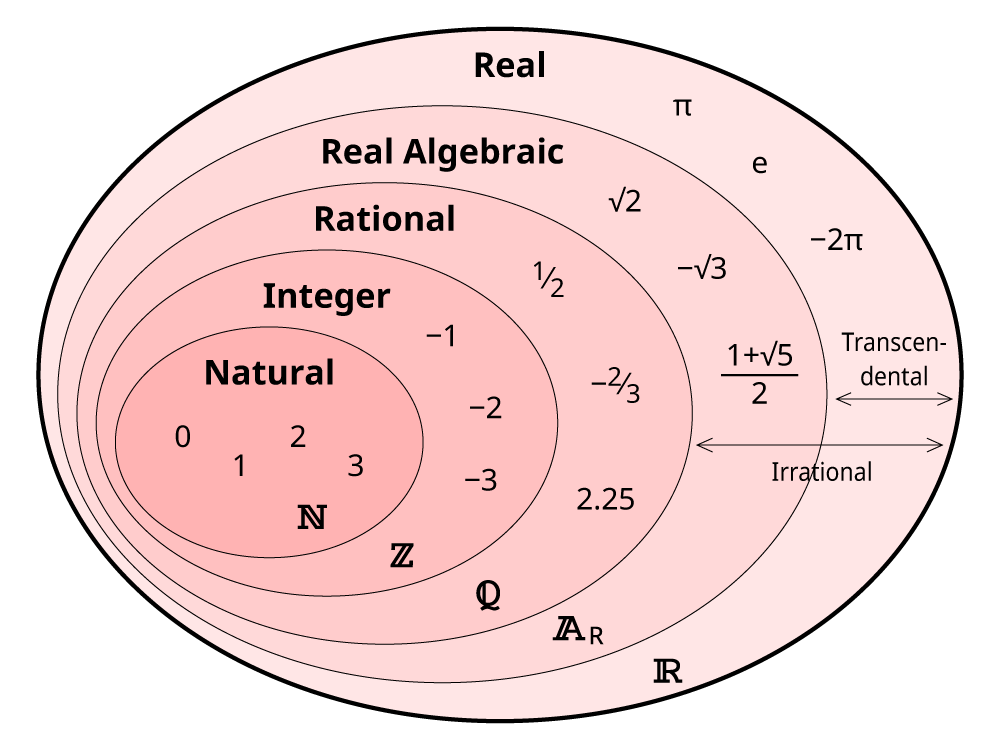
\includegraphics[width=\textwidth/2]{numbers set.png}
	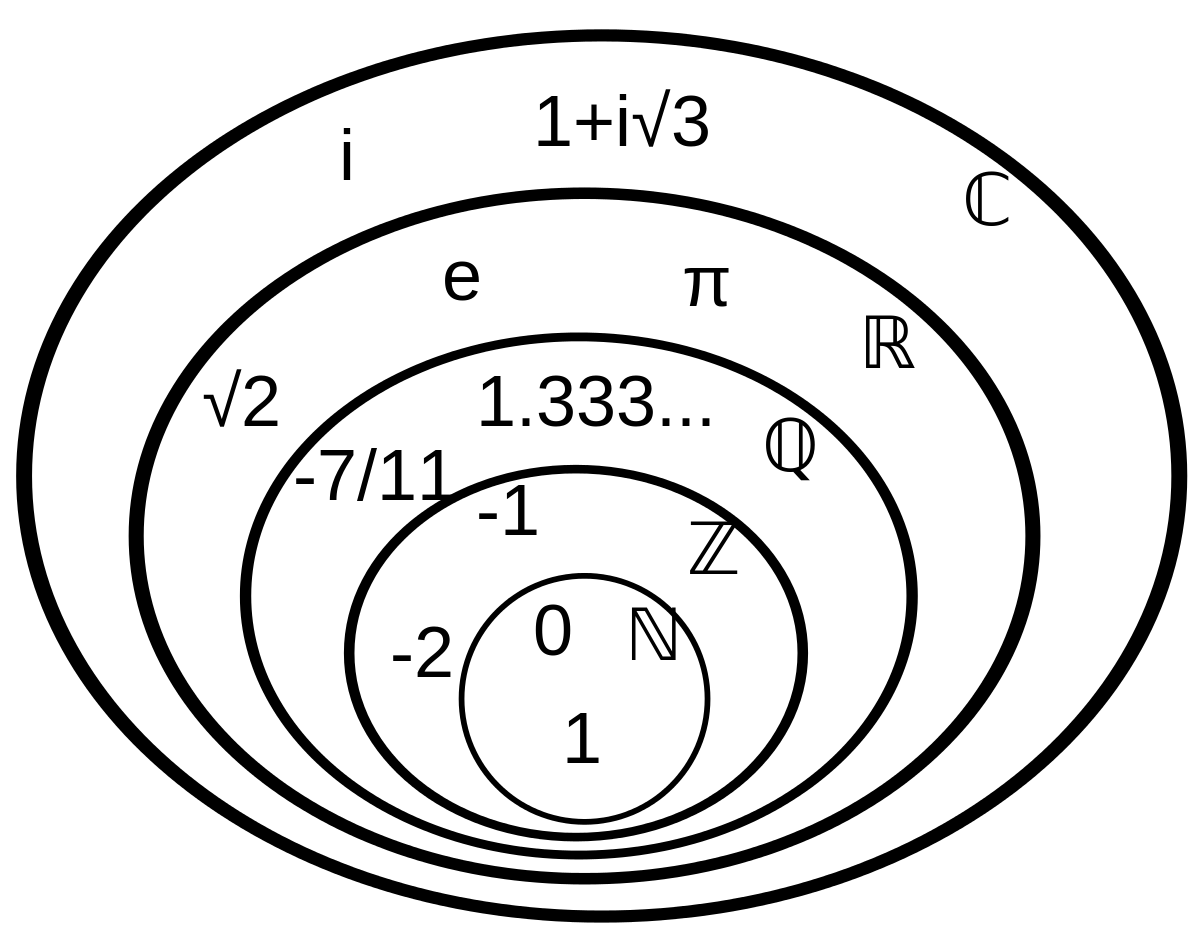
\includegraphics[width=\textwidth/2]{compset.png}
	\caption{dari: https://thinkzone.wlonk.com/Numbers/RealSet\_w1000.png}
	\caption{dan https://en.wikipedia.org/wiki/Number}
	\end{figure}
	
	\begin{enumerate}
	\item $\NN$ adalah himpunan bilangan asli (Natural Numbers) $\{1,2,3,\dots\}$. Di beberapa negara Eropa dan beberapa negara lain, himpunan bilangan asli adalah $\{0,1,2,\dots\}$.
	\item $\ZZ$ adalah himpunan bilangan bulat $\ZZ=\{\dots,-2,-1,0,1,2,\dots\}$.
	\item $\QQ$ adalah himpunan bilangan rasional, dengan definisi $\QQ=\{\dfrac{a}{b}\mid a\in \ZZ, b\in\ZZ^+\}$.
	\item $\RR$ adalah himpunan bilangan real, semua bilangan yang ada di dunia nyata, termasuk bilangan irasional seperti $\sqrt{2}$ dan rasional.
	\item $\CC$ adalah himpunan bilangan kompleks dengan definisi\\ $\CC = \{a+bi \mid a,b \in \RR \text{ dan }i=\sqrt{-1}\}$.
	\item Definisikan pula $\ZZ^+$ sebagai himpunan bialangan bulat positif. Aturan yang sama juga berlaku: $\RR^+, \QQ^+$.
	\end{enumerate}
	

	
	\section{Aljabar}
	\subsection{Pemfaktoran dan Penguraian}
	Pelajaran dari SMP ini mahh. Jangan dihafal secara sengaja, tetapi banyak-banyaklah latihan soal, nanti hafal sendiri :D.
	
	Untuk $x,y,z \in \CC$.
	\begin{enumerate}
	    \item $x^2-y^2 = (x+y)(x-y)$.
	    \item $(x+y)^2 = x^2+2xy+y^2$.
	    \item $(x+y+z)^2 = x^2+y^2+z^2+2xy+2yz+2zx$.
	    \item $(x-y)^2 = x^2-2xy+y^2$.
	    \item $x^3-y^3 = (x-y)(x^2+xy+y^2)$.
	    \item $x^3+y^3 = (x+y)(x^2-xy+y^2)$.
	    \item $(x+y)^3 = x^3+y^3+3xy(x+y) = x^3+3x^2y+3xy^2+y^3$. 
	    \item $(x-y)^3 = x^3-y^3+3xy(x-y) = x^3-3x^2y+3xy^2-y^3$. 
	    \item $x^n-y^n = (x-y)(x^{n-1}+x^{n-2}y+x^{n-3}y^2+\dots+xy^{n-2}+y^{n-1})$ untuk $n \in \NN$.
	    \item $x^n+y^n = (x+y)(x^{n-1}-x^{n-2}y+x^{n-3}y^2-\dots+xy^{n-2}+y^{n-1})$ untuk $n$ adalah bilangan asli \textbf{ganjil}.
	    \item $x^2+y^2+z^2+xy+yz+zx = \frac12(x+y)^2+\frac12(y+z)^2+\frac12(z+x)^2$.
	    \item $x^2+y^2+z^2-xy-yz-zx = \frac12(x-y)^2+\frac12(y-z)^2+\frac12(z-x)^2$.
	    \item $x^3+y^3+z^3-3xyz = (x+y+z)(x^2+y^2+z^2-xy-yz-zx)$.
	    \item $(x+1)(y+1)(z+1)=xyz+xy+yz+zx+x+y+z+1$.
	    \item (Identitas Sophie Germain) $x^4+4y^4=(x^2+2xy+2y^2)(x^2-2xy+2y^2)$.
	    \item (Ekspansi Binomial) $(x+y)^n = {n \choose 0}x^ny^0 + {n \choose 1}x^{n-1}y^1+{n \choose 2}x^{n-2}y^2 + \dots + {n \choose n}x^0y^n$.
	    \item (Fermat Two Square Identity) $(a^2+b^2)(c^2+d^2)=(bc+ad)^2+(bd-ac)^2$ untuk $a,b,c,d \in \RR$.
	\end{enumerate}
	
	\section{Teori Bilangan}
	Pada dasarnya aljabar tetapi di ranah bilangan bulat (atau rasional).
	\subsection{Sifat-sifat Penjumlahan dan Perkalian Dua Bilangan Bulat}
    \begin{enumerate}
        \item Bilangan Ganjil ± Bilangan Ganjil = Bilangan Genap 
        \item Bilangan Ganjil ± Bilangan Genap = Bilangan Ganjil 
        \item Bilangan Genap ± Bilangan Ganjil = Bilangan Ganjil 
        \item Bilangan Genap ± Bilangan Genap = Bilangan Genap 
        \item Bilangan Ganjil $\times$ Bilangan Ganjil = Bilangan Ganjil 
        \item Bilangan Ganjil $\times$ Bilangan Genap = Bilangan Genap 
        \item Bilangan Genap $\times$ Bilangan Ganjil = Bilangan Genap 
        \item Bilangan Genap $\times$ Bilangan Genap = Bilangan Genap
    \end{enumerate}
    Dari sifat-sifat perkalian dua bilangan akan didapat bahwa bilangan genap tidak mungkin membagi 
    bilangan ganjil sedangkan bilangan ganjil mungkin membagi bilangan genap. 
    \subsection{Keterbagian}
    Untuk bilangan bulat $a \neq 0$ serta bilangan bulat $b,c,x$ dan $y$, notasikan $a \mid b$ sebagai $a$ membagi $b$. Lalu, $a$ dan $b$ relatif prima atau $a$ dan $b$ koprima (coprime) jika dan hanya jika $FPB(a,b)=1$.
    \begin{enumerate}
        \item Kita dapat menyatakan semua bilangan bulat $c = pq+r$ untuk suatu bilangan bulat $q$ dimana $0 \le r < q$. Jadi, saat $c$ dibagi $p$, maka hasil baginya adalah $q$ dan sisa baginya adalah $r$.
        \item Terdapat suatu bilangan bulat $x$ dimana $a \mid b \iff b=ax$.
        \item $a \mid a$.
        \item $a \mid 0$.
        \item $1 \mid a$.
        \item $a \mid b \implies a \mid bc$.
        \item Untuk $a,b \neq 0$ maka $ab \mid c \implies a \mid c \text{ dan } b \mid c$.
        \item $a \mid b \text{ dan } b \mid c \implies a \mid c$.
        \item $a \mid b \text{ dan } a \mid c \implies a \mid bx + cy$.
        \item Untuk $x \neq 0$ maka $a \mid b \iff xa \mid xb$.
        \item $a \mid b$ dan $b \neq 0$ maka $|a| \le |b|$.
        \item $a \mid bc$ dan $FPB(a,b)=1$ maka $a\mid c$.
    \end{enumerate}
    \subsection{Uji habis dibagi}
    Trik yang suatu saat dapat membuat hidup anda bahagia wkwkwk. Semua rumus ini dapat dibuktikan dengan aritmatika modular.
    \begin{enumerate}
        \item Bilangan $x$ genap jika dan hanya jika digit terakhir $x$ genap.
        \item $3 \mid x$ jika dan hanya jika jumlah digit-digitnya habis dibagi $3$. Contohnya 2931 habis dibagi 3 karena $2+9+3+1=15$ habis dibagi 3.
        \item $9 \mid x$ jika dan hanya jika jumlah digit-digitnya habis dibagi $9$.
        \item $x$ habis dibagi 5 jika dan hanya jika digit terakhir $x$ adalah $0$ atau $5$.
        \item $x$ habis dibagi 11 jika dan hanya jika jumlah selang-seling (alternate sums) dari digit-digitnya habis dibagi 11. Contoh: 945351 habis dibagi 11 karena $9-4+5-3+5-1=11$ habis dibagi 11. 121 habis dibagi 11 karena $1-2+1=0$ habis dibagi 11.
    \end{enumerate}
    
    \subsection{Aritmatika Modular}
    Untuk suatu bilangan asli $m$ dan bilangan bulat $a,b,c$ dan $d$, notasikan $m\mid a-b \iff a \equiv b \mod m$ (dibaca $a$ kongruen $b$ modulo $m$). Simpelnya $a \equiv b \mod m$ adalah $a$ dibagi $m$ bersisa $b$. Contohnya $5 \equiv 2 \mod 3$. $13 \equiv 3 \mod 5$. $10 \equiv -2 \mod 12$.
    \begin{enumerate}
        \item $a \equiv a \mod m$.
        \item $a \equiv 0 \mod m \iff m\mid a$.
        \item $a \equiv b \mod m \iff b \equiv a \mod m$.
        \item $a \equiv b \mod m \text{ dan } b \equiv c \mod m \implies a \equiv c \mod m$.
        \item Jika $a \equiv b \mod m$ dan $d\mid m$ maka $a \equiv b \mod d$.
        \item Untuk semua bilangan asli $k$, $a \equiv b \mod m \iff a^k \equiv b^k \mod m$.
        \item $a \equiv b \mod m \text{ dan } c \equiv d \mod m \implies a+c \equiv b+d \mod m$.
        \item $a \equiv b \mod m \text{ dan } c \equiv d \mod m \implies ac \equiv bd \mod m$.
        \item $\forall k\in \ZZ^+, (am+b)^k \equiv b^k \mod m$.
        \item Jika $ca \equiv cb \mod m$ dengan $FPB(c,m)=1$, maka $a \equiv b \mod m$.
    \end{enumerate}
    
    Penggunaan sifat nomor 8 dapat dimodifikasi sehingga menjadi konsep \textbf{Chinese Remainder Theorem}.
    
    \section{Kombinatorika}
    
    Notasikan $n!=n \times (n-1) \times (n-2) \times \dots \times 3 \times 2 \times 1$ (dibaca $n$ faktorial) dengan $1!=0!=1$.
    
    \subsection{Kombinasi dan Permutasi}
    Permutasi $k$ unsur dari $n$ unsur adalah (urutan diperhatikan)
    $$_nP_K = P_k^n = \dfrac{n!}{(n-k)!}.$$
    Kombinasi $k$ unsur dari $n$ unsur adalah (urutan tak diperhatikan)
    $${n \choose k}=_nC_K = C_k^n = \dfrac{n!}{k!(n-k)!}.$$
    
    \subsection{Permutasi Siklis}
    $n$ objek ditaruh mengelilingi lingkaran maka banyak cara menyusunnya adalah
    $$P_{siklis} =\dfrac{n!}{n} = (n-1)!$$
    
    \subsection{Stars and Bars}
    Banyaknya solusi bulat non-negatif $(x_1,x_2,\dots,x_k)$ dari sistem persamaan $x_1+x_2+\dots+x_k=n$ adalah
    $${n+k-1 \choose k-1}.$$
    Banyaknya solusi bulat positif $(x_1,x_2,\dots,x_k)$ dari sistem persamaan $x_1+x_2+\dots+x_k=n$ adalah
    $${n-1 \choose k-1}.$$
    
    \section{Geometri}
    Pada dasarnya geometri di olimpiade matematika SMA "hanya" tentang lingkaran dan segitiga , "saja". 
    
    \subsection{Garis, Segmen Garis, Sinar (Bukan Vektor ya...)}
    Perlu ditekankan bahwa \textbf{garis tidak sama dengan ruas garis}. Garis panjangnya tak hingga, sedangkan ruas garis atau segmen garis panjangnya terbatas. Gambar di bawah terdiri dari \textbf{garis AB, segmen garis CD, sinar EF}.
\begin{center}
        \definecolor{ududff}{rgb}{0.30196078431372547,0.30196078431372547,1}
\begin{tikzpicture}[line cap=round,line join=round,>=triangle 45,x=1cm,y=1cm]
\clip(-9,-3) rectangle (5,5);
\draw [line width=2pt,domain=-12.65:12.65] plot(\x,{(--18.806--2.68*\x)/3.84});
\draw [line width=2pt] (-4.47,-0.96)-- (-1.65,1.26);
\draw [line width=2pt,domain=-3.19:12.649999999999997] plot(\x,{(--2.1004--2.44*\x)/2.96});
\begin{scriptsize}
\draw [fill=ududff] (-6.53,0.34) circle (2.5pt);
\draw[color=ududff] (-6.38,0.74) node {$A$};
\draw [fill=ududff] (-2.69,3.02) circle (2.5pt);
\draw[color=ududff] (-2.54,3.42) node {$B$};
\draw [fill=ududff] (-4.47,-0.96) circle (2.5pt);
\draw[color=ududff] (-4.32,-0.56) node {$C$};
\draw [fill=ududff] (-1.65,1.26) circle (2.5pt);
\draw[color=ududff] (-1.5,1.66) node {$D$};
\draw [fill=ududff] (-3.19,-1.92) circle (2.5pt);
\draw[color=ududff] (-3.04,-1.52) node {$E$};
\draw [fill=ududff] (-0.23,0.52) circle (2.5pt);
\draw[color=ududff] (-0.08,0.92) node {$F$};
\end{scriptsize}
\end{tikzpicture}
\end{center}
    
    \subsection{Lingkaran}
    
    \begin{center}
    \definecolor{ffwwqq}{rgb}{1,0.4,0}
\definecolor{uuuuuu}{rgb}{0.26666666666666666,0.26666666666666666,0.26666666666666666}
\definecolor{ffqqtt}{rgb}{1,0,0.2}
\definecolor{ttttff}{rgb}{0.2,0.2,1}
\definecolor{xdxdff}{rgb}{0.49019607843137253,0.49019607843137253,1}
\definecolor{ududff}{rgb}{0.30196078431372547,0.30196078431372547,1}
\begin{tikzpicture}[line cap=round,line join=round,>=triangle 45,x=1cm,y=1cm,scale=1.5]
\clip(-7,-2) rectangle (0,3.5);
\draw [line width=2pt] (-3.71,0.7) circle (2.64cm);
\draw [line width=1.2pt] (-1.07,0.7)-- (-5.351768859108188,2.767412637395495);
\draw [line width=0.8pt,color=ttttff] (-5.351768859108188,2.767412637395495)-- (-3.71,0.7);
\draw [line width=0.8pt,color=ttttff] (-3.71,0.7)-- (-5.909770515623599,-0.7596608094324813);
\draw [line width=1.2pt] (-5.909770515623599,-0.7596608094324813)-- (-1.07,0.7);
\draw [line width=2pt,color=xdxdff] (-5.351768859108188,2.767412637395495)-- (-6.308385428488046,1.1668973816814456);
\draw [line width=2pt,color=xdxdff] (-6.308385428488046,1.1668973816814456)-- (-5.909770515623599,-0.7596608094324813);
\draw [line width=1.2pt] (-5.351768859108188,2.767412637395495)-- (-1.3105942592998239,-0.40111402293088494);
\draw [line width=1.2pt] (-1.3105942592998239,-0.40111402293088494)-- (-5.909770515623599,-0.7596608094324813);
\draw [line width=1.2pt,color=ffqqtt] (-5.351768859108188,2.767412637395495)-- (-5.909770515623599,-0.7596608094324813);
\draw [line width=2pt,color=ffwwqq] (-3.71,0.7)-- (-5.630769687365895,1.0038759139815074);
\begin{scriptsize}
\draw [fill=ududff] (-3.71,0.7) circle (0.5pt);
\draw[color=ududff] (-3.6221931954155986,0.843846768592457) node {$O$};
\draw [fill=ududff] (-1.07,0.7) circle (0.5pt);
\draw[color=ududff] (-0.9803781371406202,0.843846768592457) node {$B$};
\draw [fill=xdxdff] (-5.351768859108188,2.767412637395495) circle (0.5pt);
\draw[color=xdxdff] (-5.476098499468215,2.9526640519523077) node {$C$};
\draw [fill=xdxdff] (-5.909770515623599,-0.7596608094324813) circle (0.5pt);
\draw[color=xdxdff] (-6.0554439069846575,-0.8246680050548971) node {$A$};
\draw [fill=xdxdff] (-6.308385428488046,1.1668973816814456) circle (0.5pt);
\draw[color=xdxdff] (-6.507333324847482,1.2493885538539669) node {$D$};
\draw [fill=xdxdff] (-1.3105942592998239,-0.40111402293088494) circle (0.5pt);
\draw[color=xdxdff] (-1.2237032082975259,-0.25690950568878346) node {$E$};
\draw [fill=uuuuuu] (-5.630769687365895,1.0038759139815074) circle (0.5pt);
\draw[color=uuuuuu] (-5.545619948370188,1.145106380501007) node {$F$};
\end{scriptsize}
\end{tikzpicture}
\end{center}
Misalkan $O$ pusat lingkaran dan $A,B,C,D,E$ adalah sembarang titik seperti gambar.
\begin{enumerate}
    \item $CO=OA$ adalah jari-jari dengan $\angle ACO = \angle OAC$.
    \item Misalkan titik $F$ adalah titik tengah tali busur $CA$, maka $OF \perp CA$ atau $OF$ tegak lurus dengan $CA$, dengan kata lain, $F$ adalah proyeksi titik $O$ ke $CA$
    \item (Sudut keliling-sudut pusat) Untuk$\angle COA = 2\angle CBA$.
    \item (sudut keliling) $\angle CBA = \angle CEA$.
    \item $ABCD$ adalah segiempat tali busur atau segiempat siklis  atau $A,B,C,D$ terletak di lingkaran (seperti pada gambar) jika dan hanya jika $\angle CBA + \angle ADC = 180^\circ$.
\end{enumerate}

\section{Segitiga}

\begin{center}
\definecolor{qqzzqq}{rgb}{0,0.6,0}
\definecolor{yqqqyq}{rgb}{0.5019607843137255,0,0.5019607843137255}
\definecolor{qqttcc}{rgb}{0,0.2,0.8}
\definecolor{uuuuuu}{rgb}{0.26666666666666666,0.26666666666666666,0.26666666666666666}
\definecolor{zzttqq}{rgb}{0.6,0.2,0}
\definecolor{ududff}{rgb}{0.30196078431372547,0.30196078431372547,1}
\begin{tikzpicture}[line cap=round,line join=round,>=triangle 45,x=1cm,y=1cm,scale=2]
\clip(-7.9,-3.2) rectangle (0,3.2);
\fill[line width=2pt,color=zzttqq,fill=zzttqq,fill opacity=0.10000000149011612] (-6.165519534412781,1.8403208695207385) -- (-6.617408952275606,-1.1954490658654202) -- (-0.9745846830654554,-1.1722752495647626) -- cycle;
\fill[line width=2pt,color=zzttqq,fill=zzttqq,fill opacity=0.10000000149011612] (-6.165519534412781,1.8403208695207385) -- (-6.617408952275606,-1.1954490658654202) -- (-0.9745846830654554,-1.1722752495647626) -- cycle;
\draw [line width=2pt,color=zzttqq] (-6.165519534412781,1.8403208695207385)-- (-6.617408952275606,-1.1954490658654202);
\draw [line width=2pt,color=zzttqq] (-6.617408952275606,-1.1954490658654202)-- (-0.9745846830654554,-1.1722752495647626);
\draw [line width=2pt,color=zzttqq] (-0.9745846830654554,-1.1722752495647626)-- (-6.165519534412781,1.8403208695207385);
\draw [line width=1.2pt,domain=-8.957964398642034:-0.18667492884309483] 
\draw [line width=1.2pt,color=qqttcc] (-6.165519534412781,1.8403208695207385)-- (-4.708133684869424,-1.1876080996748404);
\draw [line width=1.2pt,color=yqqqyq] (-6.165519534412781,1.8403208695207385)-- (-6.153060138278336,-1.193542089216561);
\draw [line width=2pt,color=zzttqq] (-6.165519534412781,1.8403208695207385)-- (-6.617408952275606,-1.1954490658654202);
\draw [line width=2pt,color=zzttqq] (-6.617408952275606,-1.1954490658654202)-- (-0.9745846830654554,-1.1722752495647626);
\draw [line width=2pt,color=zzttqq] (-0.9745846830654554,-1.1722752495647626)-- (-6.165519534412781,1.8403208695207385);
\draw [line width=2pt] (-3.8005990144458206,-0.06322724293202202) circle (3.035843290122741cm);
\draw [line width=2pt] (-5.267050752412224,-0.02637740656707221) circle (1.1635162287432892cm);
\draw [line width=1.2pt,color=qqzzqq] (-6.165519534412781,1.8403208695207385)-- (-3.795996817670531,-1.1838621577150916);
\begin{scriptsize}
\draw [fill=ududff] (-6.165519534412781,1.8403208695207385) circle (0.5pt);
\draw[color=ududff] (-6.078617723285315,1.9793637673246847) node {$A$};
\draw [fill=ududff] (-6.617408952275606,-1.1954490658654202) circle (0.5pt);
\draw[color=ududff] (-6.5305071411481395,-1.0564061680614731) node {$B$};
\draw [fill=ududff] (-0.9745846830654554,-1.1722752495647626) circle (0.5pt);
\draw[color=ududff] (-0.8876828719379902,-1.0332323517608155) node {$C$};
\draw [fill=uuuuuu] (-6.153060138278336,-1.193542089216561) circle (0.5pt);
\draw[color=uuuuuu] (-6.182899896638275,-1.2765574229177212) node {$D$};
\draw [fill=uuuuuu] (-4.708133684869424,-1.1876080996748404) circle (0.5pt);
\draw[color=uuuuuu] (-4.6186672963438795,-1.0448192599111443) node {$E$};
\draw [fill=uuuuuu] (-3.795996817670531,-1.1838621577150916) circle (0.5pt);
\draw[color=uuuuuu] (-3.703301552467901,-1.0448192599111443) node {$M$};
\draw[color=black] (-5.841086106203574,2.5934698992921135) node {$L1$};
\draw [fill=uuuuuu] (-3.800599014445821,-0.06322724293202069) circle (0.5pt);
\draw[color=uuuuuu] (-3.5758455628142833,-0.0831058834338501) node {$O$};
\draw [fill=uuuuuu] (-5.267050752412224,-0.02637740656707221) circle (0.5pt);
\draw[color=uuuuuu] (-5.174838887559664,0.11387155512174028) node {$I$};
\draw[color=black] (-5.87584683065456,0.8554336767427865) node {$L2$};
\draw [fill=uuuuuu] (-6.156315140862202,-0.40094896004539987) circle (0.5pt);
\draw[color=uuuuuu] (-6.067030815134986,-0.25690950568878285) node {$H$};
\end{scriptsize}
\end{tikzpicture}
\end{center}
Pada segitiga $ABC$,
\begin{enumerate}
    \item Berlaku \textbf{ketaksamaan segitiga} yaitu $AB+BC>CA$, $BC+CA>AB$, dan $CA+AB>BC$. Selain itu juga berlaku $|AB-BC|<CA$, $|BC-CA|<AB$, dan $|CA-AB|<BC$.
    \item Garis bagi $AE$ yaitu garis yang membagi dua sudut $A$ sama besar sehingga $\angle BAE = \angle EAC$. Berlaku \textbf{Teorema Garis Bagi}, yaitu $\dfrac{AB}{AC}=\dfrac{BE}{CE}$.
    \item Garis berat $AM$ dengan $M$ adalah titik tengah $BC$.
    \item Garis tinggi $AD$ adalah garis yang tegak lurus dengan $BC$. $D$ biasa disebut dengan proyeksi $A$ ke $BC$.
    \item Garis $OM$ adalah salah satu garis sumbu segitiga $ABC$, yaitu garis yang melewati titik tengah sisi segitiga dan tegak lurus dengan sisi itu.
    \item Pertemuan atau perpotongan ketiga garis tinggi segitiga $ABC$ adalah titik tinggi, dalam gambar ini adalah $H$ (orthocenter).
    \item Pertemuan atau perpotongan ketiga garis bagi segitiga $ABC$ adalah titik bagi atau titik pusat lingkaran dalam (incircle $L2$) segitiga $ABC$ dalam gambar ini adalah $I$ (incenter).
    \item Pertemuan atau perpotongan ketiga garis berat segitiga $ABC$ adalah titik berat (centroid).
    \item Pertemuan atau perpotongan ketiga garis sumbu segitiga $ABC$ adalah titik pusat lingkaran luar (circumcircle $L1$) segitiga $ABC$ yang dalam gambar ini adalah $O$ (circumcenter).
\end{enumerate}

\subsection{Kesebangunan Segitiga}
\begin{center}
\definecolor{xdxdff}{rgb}{0.49019607843137253,0.49019607843137253,1}
\definecolor{ttttff}{rgb}{0.2,0.2,1}
\definecolor{qqzzff}{rgb}{0,0.6,1}
\definecolor{ududff}{rgb}{0.30196078431372547,0.30196078431372547,1}
\begin{tikzpicture}[line cap=round,line join=round,>=triangle 45,x=1cm,y=1cm]
\clip(-6.5,0.5) rectangle (0.5,4);
\fill[line width=2pt,color=qqzzff,fill=qqzzff,fill opacity=0.1] (-5.933781371406205,1.3073230946056116) -- (-5.37760978019042,2.72092588894573) -- (-3.76702954729471,1.3420838190565978) -- cycle;
\fill[line width=0.8pt,color=xdxdff,fill=xdxdff,fill opacity=0.1] (-3.1992710479285953,0.9944765745467326) -- (-2.283905304052617,3.2307498475601983) -- (0.299975213470717,1.0524111152983768) -- cycle;
\draw [line width=2pt,color=qqzzff] (-5.933781371406205,1.3073230946056116)-- (-5.37760978019042,2.72092588894573);
\draw [line width=2pt,color=qqzzff] (-5.37760978019042,2.72092588894573)-- (-3.76702954729471,1.3420838190565978);
\draw [line width=2pt,color=qqzzff] (-3.76702954729471,1.3420838190565978)-- (-5.933781371406205,1.3073230946056116);
\draw [line width=0.8pt,color=xdxdff] (-3.1992710479285953,0.9944765745467326)-- (-2.283905304052617,3.2307498475601983);
\draw [line width=0.8pt,color=xdxdff] (-2.283905304052617,3.2307498475601983)-- (0.299975213470717,1.0524111152983768);
\draw [line width=0.8pt,color=xdxdff] (0.299975213470717,1.0524111152983768)-- (-3.1992710479285953,0.9944765745467326);
\begin{scriptsize}
\draw [fill=ududff] (-5.933781371406205,1.3073230946056116) circle (0.5pt);
\draw[color=ududff] (-5.846879560278738,1.4463659924095578) node {$A$};
\draw [fill=ududff] (-5.37760978019042,2.72092588894573) circle (0.5pt);
\draw[color=ududff] (-5.290707969062953,2.859968786749677) node {$B$};
\draw [fill=ududff] (-3.76702954729471,1.3420838190565978) circle (0.5pt);
\draw[color=ududff] (-3.6801277361672433,1.4811267168605442) node {$C$};
\draw [fill=ududff] (-3.1992710479285953,0.9944765745467326) circle (0.5pt);
\draw[color=ududff] (-3.1123692368011295,1.133519472350679) node {$D$};
\draw [fill=ududff] (-2.283905304052617,3.2307498475601983) circle (0.5pt);
\draw[color=ududff] (-2.1970034929251505,3.3697927453641463) node {$E$};
\draw [fill=ttttff] (0.299975213470717,1.0524111152983768) circle (0.5pt);
\draw[color=ttttff] (0.38687702459818324,1.191454013102323) node {$F$};
\end{scriptsize}
\end{tikzpicture}
\end{center}

Segitiga $ABC$ dan $DEF$ sebangun atau $ABC \sim DEF$ jika dan hanya jika minimal salah satu syarat ini terpenuhi:
\begin{enumerate}
    \item $\angle ABC = \angle DEF$ dan $\angle BAC = \angle EDF$.
    \item $\dfrac{AB}{DE} = \dfrac{BC}{EF} = \dfrac{CA}{FD}$.
    \item $\dfrac{AB}{DE} = \dfrac{BC}{EF}$ dan $\angle ABC = \angle DEF$ (sudut yang diapit dua sisi yang diperbandingkan nilainya sama)
\end{enumerate}

\subsection{Kekongruenan Segitiga}
\begin{center}
\definecolor{xdxdff}{rgb}{0.49019607843137253,0.49019607843137253,1}
\definecolor{ttttff}{rgb}{0.2,0.2,1}
\definecolor{qqzzff}{rgb}{0,0.6,1}
\definecolor{ududff}{rgb}{0.30196078431372547,0.30196078431372547,1}
\begin{tikzpicture}[line cap=round,line join=round,>=triangle 45,x=1cm,y=1cm]
\clip(-8,0.5) rectangle (0.5,4);
\fill[line width=2pt,color=qqzzff,fill=qqzzff,fill opacity=0.1] (-7.671817593955533,1.110345656050021) -- (-6.756451850079554,3.3582058372138173) -- (-4.184158240706549,1.1914540131023228) -- cycle;
\fill[line width=0.8pt,color=xdxdff,fill=xdxdff,fill opacity=0.1] (-3.8828986287979985,1.191454013102323) -- (-2.9675328849220186,3.4277272861157897) -- (-0.38365236739868475,1.2493885538539673) -- cycle;
\draw [line width=2pt,color=qqzzff] (-7.671817593955533,1.110345656050021)-- (-6.756451850079554,3.3582058372138173);
\draw [line width=2pt,color=qqzzff] (-6.756451850079554,3.3582058372138173)-- (-4.184158240706549,1.1914540131023228);
\draw [line width=2pt,color=qqzzff] (-4.184158240706549,1.1914540131023228)-- (-7.671817593955533,1.110345656050021);
\draw [line width=0.8pt,color=xdxdff] (-3.8828986287979985,1.191454013102323)-- (-2.9675328849220186,3.4277272861157897);
\draw [line width=0.8pt,color=xdxdff] (-2.9675328849220186,3.4277272861157897)-- (-0.38365236739868475,1.2493885538539673);
\draw [line width=0.8pt,color=xdxdff] (-0.38365236739868475,1.2493885538539673)-- (-3.8828986287979985,1.191454013102323);
\begin{scriptsize}
\draw [fill=ududff] (-7.671817593955533,1.110345656050021) circle (0.5pt);
\draw[color=ududff] (-7.584915782828065,1.2493885538539673) node {$A$};
\draw [fill=ududff] (-6.756451850079554,3.3582058372138173) circle (0.5pt);
\draw[color=ududff] (-6.669550038952086,3.4972487350177635) node {$B$};
\draw [fill=ududff] (-4.184158240706549,1.1914540131023228) circle (0.5pt);
\draw[color=ududff] (-4.097256429579081,1.3304969109062692) node {$C$};
\draw [fill=ududff] (-3.8828986287979985,1.191454013102323) circle (0.5pt);
\draw[color=ududff] (-3.7959968176705314,1.3304969109062692) node {$D$};
\draw [fill=ududff] (-2.9675328849220186,3.4277272861157897) circle (0.5pt);
\draw[color=ududff] (-2.8806310737945524,3.5667701839197368) node {$E$};
\draw [fill=ttttff] (-0.38365236739868475,1.2493885538539673) circle (0.5pt);
\draw[color=ttttff] (-0.29675055627121893,1.3884314516579135) node {$F$};
\end{scriptsize}
\end{tikzpicture}
\end{center}
Sedangkan $ABC$ dan $DEF$ dikatakan kongruen atau $\triangle ABC \cong \triangle DEF$ jika dan hanya jika $AB=DE, BC=EF, CA=FD$ atau dengan kata lain kedua segitiga tersebut sebangun dan ada salah satu sisi dari kedua segitiga tersebut yang panjangnya sama. Simpelnya kongruen = sama persis.

\subsection{Trigonometri}
Banyak sih rumusnya, tapi yang paling sering dipake di olim:
\begin{enumerate}
    \item $\sin (-x) = -\sin x$.
    \item $\cos (-x) = \cos x$.
    \item $\tan(-x) = -\tan x$.
    \item $\sin^2 x + \cos^2 x = 1$.
    \item $\sin(90^\circ-x)=\sin(90^\circ+x)=\cos x$.
    \item $\sin(a \pm b) = \sin a \cos b \pm \cos a \sin b$.
    \item $\sin 2x = 2\sin x \cos x$.
    \item $\cos(a \pm b) = \cos a \cos b \mp \sin a \sin b$.
    \item $\cos 2x = \cos^2 x - \sin^2 x = 2\cos^2 x -1 = 1-2\sin^2 x$.
    \item $\tan(a \pm b) = \dfrac{\tan a \pm \tan b}{1 \mp \tan a \tan b}$.
\end{enumerate}
Cara menghafal yang gampang bisa make "metode sumbu" (ask me on training to knows more)
\section{Latihan Soal}
\subsection{Aljabar}
\begin{enumerate}
    \item Jika $x=2021^3-2019^3$, maka nilai $\sqrt{\dfrac{x-2}{6}}$ adalah \dots
    \item  dari $\sqrt{5050^2-4950^2}$ adalah \dots

    \item (OSP 2008) Jika $0 < b < a$ dan $a^2+b^2=6ab$, maka nilai $\dfrac{a+b}{a-b}=\dots$
    
    \item Jika $x > 0$ dan $x + \dfrac{1}{x} =  5$, maka nilai $x^3+\dfrac{1}{x^3}$ adalah \dots
    
    \item (OSK 2017) Diketahui $x-y=10$ dan $xy=10$. Nilai $x^4+y^4$ adalah \dots
    
    \item Jika $a+b+c=0$, buktikan bahwa $a^3+b^3+c^3=3abc$.

    \item (AIME 1987)
    Tentukan nilai sederhana dari $\dfrac{(10^4+324)(22^4+324)(34^4+324)(46^4+324)(58^4+324)}{(4^4+324)(16^4+324)(28^4+324)(40^4+324)(52^4+324)}$
\end{enumerate}


\subsection{Teori Bilangan}
\begin{enumerate}
    \item (OSN SMP 2003) Buktikan bahwa $(n-1)n(n^3+1)$ selalu habis dibagi 6 untuk semua bilangan asli $n$.
    
    \item Carilah semua bilangan bulat $n$ sehingga $\dfrac{2n+6}{n-1}$ adalah bilangan bulat.
    
    \item (OSK 2002) Bilangan asli $n$ terbesar sehingga $8^n \mid 44^{44}$ adalah \dots
    
    \item Berapa banyak pasangan bilangan bulat positif $(a,b)$ yang memenuhi $\dfrac{1}{a}+\dfrac{1}{b}=\dfrac{1}{6}$.
    
    \item Jika $a$ dan $b$ adalah bilangan bulat sedemikian sehingga $a^2-b^2=2017$, maka nilai dari $a^2+b^2$ adalah \dots
    
    \item (AIME 1986) Tentukan bilangan asli $n$ terbesar sehingga $n+10 \mid n^3+100$.
    
    \item (OSK 2010) Nilai $n$ terkecil sehingga $\underbrace{20102010\dots2010}_\text{$n$ buah 2010}$ habis dibagi 99 adalah \dots
    
    \item Jika dihitung maka didapat $17! = 3a56874280b6000$. Tentukan nilai digit $a$ dan $b$.
    
    \item Tentukan digit satuan dari $7^{7^7}$.
    
    \item Jika $S=1!+2!+3!+\dots+2021!$, tentukan sisa $S$ saat dibagi 6.
    
    \item (OSK 2009) Sisa saat $10^{999999999}$ saat dibagi oleh 7 adalah \dots
    \item (OSK 2011) Bilangan asli terkecil $n>2011$ yang bersisa 1 jika dibagi $2,3,4,5,6,7,8,9,10$ adalah \dots.
\end{enumerate}

\subsection{Kombinatorika}
\begin{enumerate}
    \item Misalkan terdapat 3 buah celana dan 4 buah baju. Permasalahannya adalah ada berapa banyak cara 
seseorang memilih celana dan baju yang akan dipakai ?

    \item Berapa banyak cara menyusun huruf-huruf R, A, J, I, N jika 
\begin{enumerate}
    \item huruf pertama dimulai dari huruf hidup (vokal) 
    \item huruf pertama dimulai dari huruf mati (konsonan) 
\end{enumerate}

    \item Sembilan orang siswa akan duduk pada 5 kursi sejajar. Ada berapa cara susunan mereka ? 
    
    \item Denny akan membentuk bilangan genap 3 angka yang angka-angkanya diambil dari 2, 3, 4, 5, 6, 7, 8. 
Berapa banyak bilangan yang dapat dibentuk jika : 
    \begin{enumerate}
        \item angka-angkanya boleh berulang 
\item angka-angkanya tidak boleh berulang
    \end{enumerate}
    
    \item (OSK 2003) Ada berapa banyak bilangan 4-angka (digit) yang semua angkanya genap dan bukan 
merupakan kelipatan 2003 ?
    \item  Carilah banyaknya menempatkan 3 benteng (rooks) pada papan catur $5 \times 5$ sehingga
tidak ada dua catur yang dalam posisi dapat saling menyerang.

    \item Sekumpulan orang duduk mengelilingi sebuah meja bundar. Diketahui ada 7 wanita
dimana di sebelah kanan setiap wanita tersebut adalah wanita dan ada 12 wanita yang di
sebelah kanan setiap wanita tersebut adalah pria. Diketahui pula bahwa 3 dari 4 pria di
sebelah kanannya adalah wanita. Berapa orang yang duduk mengelilingi meja tersebut?

    \item Carilah banyaknya kuadrupel terurut bilangan ganjil positif $(x_1, x_2, x_3, x_4)$ yang memenuhi
$x_1 + x_2 + x_3 + x_4 = 98$.

    \item Perhatikan gambar berikut.\\
    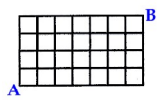
\includegraphics[scale=1.2]{kombin.PNG}
    Jika seseorang akan berjalan dari titik A ke titik B. Ada berapa banyak cara jalan terpendek 
yang dapat dipilihnya ?
    
    \item (OSP 2003) Empat pasang suami istri menonton pagelaran orkestra. Tempat duduk mereka harus 
dipisah antara kelompok suami dan kelompok istri. Untuk masing-masing kelompok disediakan 4
buah tempat duduk bersebelahan dalam satu barisan. Ada berapa banyak cara memberikan 
tempat duduk kepada mereka ?

    \item (OSK 2010) Banyaknya himpunan $X$ yang memenuhi 
$$\{1,2,\dots,1000\} \subseteq X \subseteq \{1,2,\dots,2010\}.$$

    \item (OSP 2010) Bilangan enam digit $abcdef$ dengan $a > b > c \ge d > e > f$ ada sebanyak \dots
    
    \item (OSK 2017)
	Sebuah hotel mempunyai kamar bernomor 000 sampai dengan 999. Hotel tersebut menerapkan
aturan aneh sebagai berikut: jika suatu kamar berisi tamu, dan sembarang dua digit nomor kamar
tersebut dipertukarkan tempatnya, maka diperoleh nomor kamar yang sama atau nomor kamar
yang tidak berisi tamu. Maksimal banyaknya kamar yang berisi tamu adalah \dots
\end{enumerate}

\subsection{Geometri}
\begin{enumerate}
    \item Pada segiempat $WXYZ$ dengan diagonal yang saling tegak lurus diketahui bahwa $\angle WZX = 30^\circ, \angle XWY = 40^\circ,$ and $\angle WYZ = 50^\circ$. Hitunglah besar $\angle X$ dan $\angle Z$.
    
    \item
		Garis berat $AD$ pada segitiga $ABC$ memotong garis berat $CF$ di titik $P$, serta perpanjangan $BP$ memotong $AC$ di $E$. Jika diketahui segitiga $ABC$ lancip dan $AB=6$, maka panjang $DE$ adalah \dots
		
	\item (OSK 2013) Diberikan segitiga lancip $ABC$ dengan $O$ sebagai pusat lingkaran luarnya. Misalkan $M$ dan $N$
berturut - turut pertengahan $OA$ dan $BC$. Jika $\angle ABC = 4\angle OMN$ dan $\angle ACB = 6\angle OMN$,
maka besarnya $\angle OMN$ sama dengan \dots

    \item (\textbf{Soal Legend: OSK 2011,2012,2013,2018}) Diberikan segitiga $ABC$ dan lingkaran $\Gamma$ yang berdiameter $AB$ . Lingkaran $\Gamma$ memotong sisi $AC$ dan $BC$
berturut-turut di titik $D$ dan $E$. Jika $AD = \frac13 AC, BE =\frac14 BC$ dan $AB = 30$, maka luas segitiga $ABC$ adalah \dots
		
	\item
		Diberikan segitiga $ABC$ dengan $D$ titik tengah $AC$, $E$ titik tengah $BD$, dan $H$ merupakan pencerminan $A$ terhadap $E$. Jika $F$ merupakan perpotongan antara $AH$ dengan $BC$, maka nilai $\dfrac{AF}{FH}$ sama dengan \dots
		
	\item 	
		 Pada gambar di bawah, diketahui titik A $\ne$ B pada lingkaran berdiameter $MN$ dan berpusat di $C$. $P$ adalah titik pada segmen $CN$ dimana $\angle CAP = \angle CBP = 10 ^\circ$. Jika $\angle ACM = 40^\circ$, maka $\angle BCN = \dots^\circ$
		 
		 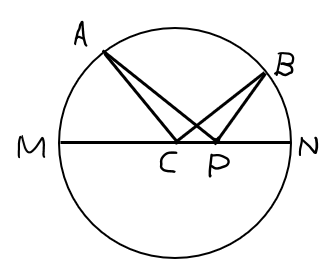
\includegraphics[scale=0.7]{pemanasan post test geom}
		 
	\item
		Diberikan sebuah segitiga dengan panjang sisi $BC = 20$, $CA = 24$, dan $AB=12$. Titik $D$ pada segmen $BC$ dengan $BD = 5$. Lingkaran luar dari segitiga $ABD$ memotong $CA$ di $E$. Hitunglah nilai $2 \times DE$.
		
	\item Jika $A+B=45^\circ$ dan $\cos A\sin B=\frac{\sqrt{2}}{6}$, maka $\cos(B-A)=\dots$
	
	\item Nilai dari $\cos \dfrac{\pi}{7}\cdot \cos \dfrac{2\pi}{7} \cdot \cos \dfrac{4\pi}{7}$ adalah \dots
	
	\item Pada segitiga $ABC$, buktikan bahwa $\tan A + \tan B + \tan C = \tan A \tan B \tan C$.
	
	\item Tentukan nilai eksak dari $\tan 1^\circ \cdot \tan 2^\circ \cdot \tan 3^\circ \cdot \ldots \cdot \tan 89^\circ$.
	
	\item (OSK 2005) Nilai dari $\sin^8 75^\circ - \cos^8 75^\circ$ adalah \dots
\end{enumerate}

%Basic 2
\graphicspath{{./}}

\section{Aljabar}
    \subsection{Barisan dan Deret}
    Simpelnya, \textbf{barisan} adalah kumpulan bilangan $a_1,a_2,\dots,a_n$ (beberapa buku atau author memulai dari $a_1$ namun ada juga yang memulai dari $a_0$, kita pakai yang dari $a_1$) yang memenuhi properti atau pola tertentu, sedangkan \textbf{deret} adalah jumlah bilangan-bilangan barisan tadi yaitu $a_1+a_1+a_2+\dots+a_n$ untuk suatu bilangan bulat non-negatif $n$.
    
    Barisan dan deret di atas adalah barisan dan deret terbatas. Bagaimana dengan barisan dan deret tak hingga? Observasi saja nilai $n$ yang sangat besar, atau dapat dikatakan ambil $n \rightarrow \infty.$
    
    \textbf{Sekali lagi barisan (bilangan-bilangan) $\neq$ deret (jumlah).}
    
    Untuk anak SMP (dan SMA) barisan dan deret paling familiar adalah barisan dan deret aritmatika serta geometri. Untuk tantangan, kerjakan latihan soal.
    
    \subsubsection{Notasi Sigma dan Pi}
    Jumlah dari suku-suku pada suatu barisan dinotasikan dengan huruf sigma kapital:
    $$\sum_{i=k}^{j} a_i = a_k+a_{k+1}+\dots+a_j.$$
    Perkalian dari suku-suku pada suatu barisan dinotasikan dengan huruf pi kapital:
    $$\prod_{i=k}^{j} a_i = a_k \cdot a_{k+1}\cdot \ldots \cdot a_j.$$
    
    Ada juga $cyc$ sebagai notasi siklis dan $sym$ sebagai notasi simetris.
    
    Misalkan kita akan mengevaluasi jumlah siklis dan simetris dari $a,b,c$.
    
    Penjumlahan bersifat \textbf{siklis} apabila setiap suku tersebut dapat diperoleh dengan "menggeser" secara siklis atau "memutar" suku lainnya.
    Contoh: $$\sum_{cyc} a = a+b+c$$
         $$\sum_{cyc} ab = ab+ bc + ca$$
    Sedikit mirip dengan penjumlahan siklis, suatu penjumlahan bersifat \textbf{simetris} apabila setiap suku dapat diperoleh dari permutasi $n$ variabel dari suku-suku lainnya pada penjumlahan. Contoh: 
        $$\sum_{sym} a = a+b+c$$
        $$\sum_{sym} ab = ab+ ac + ba + bc + ca + cb$$
    
    
    \subsubsection{Barisan dan Deret Aritmatika}
    Barisan aritmatika in a nutshell: $a,a+b,a+2b,\dots$ dimana setiap \textbf{suku ke-$n$} dari barisan tersebut adalah $$a_n=a+(n-1)b$$ untuk suatu bilangan asli $n$ dan bilangan \textbf{real} $a,b$.
    
    Lalu, \textbf{rumus deret}nya atau jumlah $n$ suku pertama barisan tersebut adalah (coba buktikan rumus ini) $$S_n = a_1+a_2+\dots+a_n=a+(a+b)+(a+2b)+\dots+(a+(n-1)b)=\dfrac{n}{2}(2a+(n-1)b).$$
    
    \subsubsection{Barisan dan Deret Geometri}
     Barisan geometri in a nutshell: $a,ar,ar^2,\dots$ dimana setiap \textbf{suku ke-$n$} dari barisan tersebut adalah $$a_n=ar^{n-1}$$ untuk suatu bilangan asli $n$ dan bilangan \textbf{real} $a$ dan $r \neq 0$.
    
    Lalu, \textbf{rumus deret}nya atau jumlah $n$ suku pertama barisan tersebut adalah (coba buktikan rumus ini) $$S_n = a_1+a_2+\dots+a_n=a+ar+ar^2+\dots+ar^{n-1}=\dfrac{a(1-r^n}{1-r}.$$
    Perhatikan jika $-1 < r < 1$ maka saat $n \rightarrow \infty$ rumus deret tak hingganya menjadi (why?) $$S_\infty =  \dfrac{a}{1-r}.$$
    
    \subsubsection{Rumus Barisan dan Deret Lainnya}
    Sangat dianjurkan untuk mencoba membuktikan rumus-rumus berikut. Untuk bilangan asli $n$, kita punya
    \begin{enumerate}
        \item $1+2+\dots+n = \dfrac{n(n+1)}{2}.$
        \item $1^2+2^2+\dots+n^2 = \dfrac{n(n+1)(2n+1)}{6}.$
        \item $1^3+2^3+\dots+n^3 = \left(1+2+\dots+n\right)^2= \left(\dfrac{n(n+1)}{2}\right)^2.$
    \end{enumerate}
    
    \subsubsection{Prinsip Teleskopik}
    Pernahkah kalian melihat deret yang dapat saling menghilangkan atau bisa "dicoret"? Berikut beberapa bentuk umumnya. Untuk lebih banyak contoh, silakan lihat contoh soal.
    
    \begin{enumerate}
        \item $\sum_{i=1}^{n} (a_{i+1}-a_{i}) = (a_2-a_1)+(a_3-a_2)+\dots+(a_{n+1}-a_{n}) = a_{n+1}-a_1.$
        \item $\prod_{i=1}^{n} \dfrac{a_{i+1}}{a_i} =  \dfrac{a_2}{a_1}\cdot\dfrac{a_3}{a_2}\cdot\dfrac{a_4}{a_3}\cdot\ldots\cdot\dfrac{a_{n+1}}{a_n} = \dfrac{a_{n+1}}{a_1}.$
    \end{enumerate}
    
    \subsection{Fungsi}
    Fungsi $f : A \rightarrow B$ adalah suatu pemetaan dari $A$ ke $B$ dimana $A$ adalah domain dan $B$ adalah kodomain fungsi. Lebh lanjut, fungsi $f$ \textit{well-defined} jika untuk $\forall x \in A$ terdapat tepat satu (jadi ngga boleh ada dua) $y \in B$ sehingga $f(x)=y$. Himpunan seluruh $y$ hasil pemetaan fungsi tersebut dinamakan \textbf{range} fungsi $f$.
    
    Tips-tips mengerjakan soal fungsi adalah (tergantung domainnya)
    \begin{enumerate}
    \item Substitusi $x=0$
    \item Mengganti $x$ dengan $-x$
    \item Mmebentuk suatu bentuk yang simetris (banyak-banyak latihan soal saja biar mengerti).
    \end{enumerate}
    
    \subsubsection{Fungsi Injektif (satu-satu)}
    Definisi: Untuk setiap $x \in A$ ada tepat satu $y \in B$ sehingga $f(x)=y$. 
    Catatan: Range dari fungsi $f$ tidak perlu mencover seluruh kodomain $B$.\\
    Contoh: Dengan $f: \RR \rightarrow \RR$, $f(x)=x$, $f(x)=2x+3$, dll.\\ 
    Contoh yang bukan fungsi injektif: Dengan $f(x)=x^2$ dari real ke real, misalkan $f(x)=4$, berarti $x=2$ dan $x=-2$, padahal biar injektif harusnya $x$ cuma satu aja.
    
    \subsubsection{Fungsi Surjektif (Fungsi Onto)}
    Definisi: Untuk setiap $y \in B$ terdapat $x \in A$ sehingga $f(x)=y$. 
    Catatan: Dapat dikatakan range fungsi tersebut adalah kodomainnya juga (untuk sebagian besar kasus) atau dengan kata lain $f(x)$ "menyentuh" semua nilai yang mungkin di kodomainnya. \\
    Contoh: $f(x)=x$, $f(x)=x^3$, dll.\\
    Contoh yang bukan fungsi surjektif: $f(x)=x^4$ dari real ke real, perhatikan bahwa $f(x)$ harus "mengcover" semua nilai, namun adakah $x$ yang membuat $f(x)=-1$? Tidak ada bukan, berarti bukan fungsi surjektif.
    
    \subsubsection{Fungsi Bijektif}
    Fungsi yang injektif sekaligus surjektif.
    
    \subsection{Komposisi Fungsi}
    Simpelnya, fungsi di dalam fungsi. Untuk fungsi $f:A \rightarrow B$ dan $g:B \rightarrow C$, komposisi fungsinya adalah
    $$(g \circ f)(x) = g(f(x)).$$
    
    \subsubsection{Invers Fungsi}
    Simpelnya kebalikan fungsi. Invers dari fungsi $f: A \rightarrow B$ adalah fungsi $f^{-1} : B \rightarrow A$ dengan didefinisikan sebagai
    $$f^{-1}(f(x))=x.$$
    Dengan kata lain, kita punya $f(x)=y$ jika dan hanya jika $f^{-1}(y)=x$.
    
    \subsection{Polinomial / Suku banyak}
    Suatu polinomial real $P(x)$ yang mempunyai derajat $n$ atau $deg(P) = n$ untuk suatu bilangan bulat non negatif $n$ dinyatakan sebagai
    $$P(x)=a_nx^n+a_{n-1}x^{n-1}+\dots+a_ax+a_0$$
    untuk suatu bilangan real $a_n,a_{n-1},\dots,a_0$ dimana $a_n \neq 0$. Dari teorema fundamental aljabar, setiap polinomial $P(x)$ tersebut memiliki maksimal $n$ akar kompleks dan dapat dinyatakan dalam bentuk
    $$P(x)=a(x-x_1)(x-x_2)\dots(x-x_n)$$
    dimana $a = a_n \neq 0$ dan $x_1,x_2,\dots,x_n$ adalah penyelesaian atau akar-akar dari persamaan $P(x)=0$ atau $a(x-x_1)(x-x_2)\dots(x-x_n)=0$.
    
    Catatan: Polinomial suku-sukunya harus memiliki pangkat positif sehingga $P(x)=x^4+5x+\sqrt{2}$ adalah suatu polinomial, tetapi $P(x)=x^3+5x^2+\dfrac{5}{x^4}+\dfrac{1}{x^8}$ bukan polinomial (karena $\dfrac{1}{x^8}$ dan $\dfrac{5}{x^4}$ bukan suku yang memiliki pangkat positif.
    
    \subsubsection{Remainder Theorem}
    Remainder Theorem = Teorema Sisa.
    Sisa polinomial $P(x)$ saat dibagi $(x-a)$ adalah $P(a)$ (why?).
    Dengan kata lain kita dapat membentuk polinomial $P(x)$ menjadi
    $$P(x)=Q(x)(x-a)+P(a)$$
    untuk suatu polinomial tak nol $Q(x)$ dengan $deg(Q)<deg(P)$.
    
    \subsubsection{Factor Theorem}
    Factor Theorem = Teorema Faktor.
    Hasil bagi polinomial $P(x)$ saat dibagi $(x-a)$ adalah $0$ atau $P(a)=0$ jika dan hanya jika $(x-a)$ adalah faktor dari $P(x)$ (why?).
    Dengan kata lain kita dapat membentuk polinomial $P(x)$ menjadi
    $$P(x)=Q(x)(x-a)$$
    untuk suatu polinomial tak nol $Q(x)$ dengan $deg(Q)<deg(P)$.
    
    \subsubsection{Teorema Vieta}
    \begin{itemize}
        \item $x_1+x_2+\dots+x_n=-\dfrac{a_{n-1}}{a_n}$
        \item $x_1x_2+x_1x_3+\dots+x_{n-1}x_n=\dfrac{a_{n-2}}{a_n}$
        \item \dots
        \item $x_1x_2x_3\ldots x_n = (-1)^{n-1}\dfrac{a_{0}}{a_n}$
    \end{itemize}
    
    Contoh:
    \begin{enumerate}
    \item Untuk $ax^3+bx^2+cx+d=0$ kita punya $x_1+x_2+x_3=-\dfrac{b}{a}$, $x_1x_2+x_1x_3+x_2x_3=\dfrac{c}{a}$, dan $x_1x_2x_3=-\dfrac{d}{a}$.
    \item Untuk $ax^2+bx+c=0$ kita punya $x_1+x_2=-\dfrac{b}{a}$ dan $x_1x_2=\dfrac{c}{a}$.
    \end{enumerate}
    
    \subsubsection{Fungsi Kuadrat}
    Fungsi kuadrat atau polinomial pangkat 2 $P(x)=ax^2+bx+c$ termasuk salah satu polinomial yang memiliki derajat 2 dan mempunyai beberapa properti penting:
    \begin{enumerate}
    \item Diskriminan $D=b^2-4ac$. Hal-hal berikut adalah \textbf{akibat langsung dari rumus abc di bawah}: $D>0$ jika dan hanya jika $P(x)$ mempunyai 2 akar real berbeda,  $D=0$ jika dan hanya jika $P(x)$ mempunyai 2 akar real kembar, dan $D<0$ jika dan hanya jika $P(x)$ mempunyai akar kompleks tidak real.
    \item Rumus abc / penyelesaian umum: $x_{1,2} = \dfrac{-b \pm \sqrt{b^2-4ac}}{2a} = \dfrac{-b+\sqrt{D}}{2a}$. Perhatikan dari rumus ini dapat dibuktikan juga rumus Vieta yang sebelumnya ditunjukkan.
    \end{enumerate}
    
    
\section{Teori Bilangan}
    \subsection{FPB dan KPK dua bilangan}
    Secara matematis FPB (atau gcd - greatest common divisors) dan KPK (atau lcm - least common multiples) dari dua bilangan bulat positif $a$ dan $b$ 
    didefinisikan sebagai:
    $$FPB(a,b) = gcd(a,b) = p_1^{\min\{a_1,b_1\}}\cdot p_2^{\min\{a_2,b_2\}} \cdot \ldots \cdot p_n^{\min\{a_n,b_n\}}$$
    $$KPK(a,b) = lcm(a,b) =p_1^{\max\{a_1,b_1\}}\cdot p_2^{\max\{a_2,b_2\}} \cdot \ldots \cdot p_n^{\max\{a_n,b_n\}}$$
    dimana kedua bilangan tersebut dapat difaktorisasi prima menjadi
    $a=p_1^{a_1}\cdot p_2^{a_2}\cdot \ldots \cdot p_n^{a_n}$ dan $b=p_1^{b_1}\cdot p_2^{b_2} \cdot \ldots \cdot p_n^{b_n}$, dengan $p_1,p_2,\dots,p_n$ adalah bilangan prima berbeda, serta $a_1,a_2,\dots,a_n,b_1,b_2,\dots,b_n$ adalah bilangan bulat non-negatif.
    
    Dari definisi tersebut mudah dibuktikan bahwa
    $$FPB(a,b) \cdot KPK(a,b) = ab.$$
    
    Perlu dicatat, bahwa $a$ dan $b$ tidak boleh bernilai nol. Untuk $a,b$ yang bernilai negatif, didefinisikan $FPB(a,b) = FPB(|a|,|b|)$.
    \subsubsection{Algoritma Euclid}
    Pada dasarnya algoritma ini bertumpu pada sebuah teorema:
    $$FPB(a,b) = FPB(a,b-a)$$
    
    \subsection{Fungsi yang Melibatkan Faktor Bilangan}
    Misalkan $a$ dapat difaktorisasi prima seperti sebelumnya yaitu $a=p_1^{a_1}\cdot p_2^{a_2}\cdot \ldots \cdot p_n^{a_n}$.
    \subsubsection{Banyaknya Faktor Positif}
    Fungsi $d(a)$ didefinisikan sebagai banyaknya faktor atau pembagi positif dari $a$ dengan
    $$d(a) = (a_1+1)(a_2+1)\cdot \ldots \cdot (a_n+1).$$
    
    Contoh: Banyaknya faktor positif dari $12= 2^2 \cdot 3^1$ adalah $d(12)=(2+1)(1+1)=6$ dengan pembagi positifnya adalah $1,2,3,4,6,12$ (ada 6 faktor positif.)
    
    \subsubsection{Jumlah Faktor Positif}
    Fungsi $\sigma (a)$ didefinisikan sebagai banyaknya faktor atau pembagi positif dari $a$ dengan
    $$\sigma (a) = (p_1^0+p_1^1+p_1^2+\dots+p_1^{a_1})(p_2^0+p_2^1+p_2^2+\dots+p_2^{a_2})\cdot \ldots \cdot (p_n^0+p_n^1+p_n^2+\dots+p_n^{a_n}).$$
    
    Contoh: Jumlah faktor atau pembagi positif dari $12= 2^2 \cdot 3^1$ adalah $d(12)=(2^0+2^1+2^2)(3^0+3^1)=28$ yang setara dengan penjumlahan secara manualnya, yaitu $2^03^0+2^03^1+2^13^0+2^13^1+2^23^0+2^23^1=28.$
    
    \subsubsection{Banyaknya Bilangan Relatif Prima}
    \begin{remark*}
    	     Bilangan $b$ dikatakan relatif prima dengan $a$ jika dan hanya jika $FPB(a,b)=1$.
    	\end{remark*}
     Definisikan fungsi Euler Totient Phi $\phi(b)$ sebagai banyaknya bilangan bulat positif $n$ yang kurang dari sama dengan $b$ dimana $n$ relatif prima dengan $b$. Rumus eksplisit untuk menghitung fungsi ini adalah
    $$\phi(n) = a\left(1-\dfrac{1}{p_1}\right)\left(1-\dfrac{1}{p_2}\right)\dots\left(1-\dfrac{1}{p_n}\right).$$
    
    Contoh: $\phi(4)=4(1-\frac{1}{2})=2$ karena ada 2 bilangan yang realtif prima dengan 4, yaitu 1 dan 3.
    
    Catatan: Untuk semua bilangan prima $p$, nilai $\phi(p) = p-1$. (Silakan dibuktikan sendiri :D)
    
    \subsection{Euler's Theorem on Modulo}
    Untuk bilangan asli $a$ dan $n$ yang saling relatif prima kita punya
    $$a^{\phi(n)} \equiv 1 \mod n.$$
    
    \subsection{Fermat's Little Theorem}
    Teorema ini merupakan kasus khusus dari Euler's Theorem saat $n$ prima sehingga $\phi(n)=n-1$. Untuk bilangan prima $p$, kita punya
    $$a^{p-1} \equiv 1 \mod p.$$
    
    \subsection{Wilson's theorem}
    Untuk suatu bilangan asli $p$, kita punya $p$ adalah bilangan prima jika dan hanya jika
    $$(p-1)! \equiv -1 \mod p.$$
    
\section{Kombinatorika}
    \subsection{Binomial Newton}
    $(a+b)^n = {n \choose 0} a^nb^0 + {n \choose 1} a^{n-1}b^1+ \dots +{n \choose n}a^0b^n$
    
    
    \subsection{Pigeon Hole Principle (PHP)}
    Teorema yang dalam Bahasa Indonesia ini disebut dengan Teorema Sangkar Burung Merpati secara matematis berbunyi:
    Jika ada $kn+1$ merpati dan $n$ sangkar, maka setidaknya ada satu sagnkar yang berisi $k+1$ burung merpati.
    
    Versi lebih simpelnya adalah: jika ada $n+1$ objek yang akan dibagi ke dalam $n$ buah kotak, maka setidaknya ada 1 kotak yang berisi 2 objek.
    
    Contoh: \begin{itemize}
        \item Di dalam ruangan berisi 3 orang, pasti terdapat setidaknya 2 orang berjenis kelamin sama.
        \item Jika ada 367 orang di suatu sekolah, maka setidaknya ada dua orang diantara mereka yang tanggal lahirnya persis sama.
    \end{itemize}
    
    \subsection{Relasi Rekurensi}
    Sering disebut dengan rekursif. Intinya adalah sebuah persamaan yang melibatkan barisan $a_1, a_2, \dots , a_n$ dimana untuk mendapatkan nilai $a_k$ membutuhkan suku-suku sebelumnya $a_{k-1}, a_{k-2}, \dots,$ atau $a_1$. 
    
    Contoh paling terkenal dari persamaan rekursif adalah bilangan Fibonacci $0,1,1,2,3,5,8,13,21,\dots$ yang secara matematis didefinisikan sebagai berikut.
    \begin{align*}
        F_0 &= 0, F_1 = 1\\
        F_n &= F_{n-1}+F_{n-2} \text{ untuk } n \ge 2
    \end{align*}
    
    atau yang lebih terkenal di ranah \textit{Computer Science} adalah permasalahan \textit{Tower of Hanoi} dengan persamaan rekursifnya didefinisikan sebagai berikut.
    \begin{align*}
        T_1 &= 1 \\
        T_n &= 2T_{n-1}+1
    \end{align*}
    
    Untuk menyelesaikan soal relasi rekurensi, butuh manipulasi aljabar yang mumpuni sehingga tidak ada pendekatan selain menggunakan persamaan karakteristik atau fungsi pembangkit (tidak dibahas disini) yang dijamin berhasil.
    
    \subsubsection{Persamaan Karakteristik untuk Relasi Rekurensi Linear}
    Persamaan karakteristik berikut berlaku untuk persamaan rekursif yang linear. Persamaan karakteristik berikut berguna untuk mengubah relasi rekurensi menjadi iteratif, atau persamaan berbentuk implisit. (Jadi, untuk persamaan yang bukan linear, sebagai contoh $a_n = a_{n-1}^2 + a_{n-2}$ tidak bisa dijamin selesai dengan persamaan karakteristik yang disajikan berikut).
    Untuk persamaan rekursif
    $$a_n = c_1a_{n-1}+c_2a_{n-2}+\dots+c_da_{n-d}$$
    mempunyai persamaan karakteristik
    $$x^d-c_1x^{d-1}-c_2x^{d-2}-\dots-c_dx^0=0$$
    
    Sebagai contoh, rumus rekursif dari barisan Fibonacci di atas dapat diselesaikan menjadi 
    $$x^{n}-x^{n-1}-x^{n-2}=0 \implies x^2-x-1=0$$
    yang mempunyai dua akar, yaitu $x_1 = \dfrac{1+\sqrt{5}}{2}=\phi$ dan $x_2 = \dfrac{1-\sqrt{5}}{2}=1-\phi$ dimana $\phi$ adalah \textit{Golden Ratio}. Sadari bahwa setiap suku di barisan Fibonacci tersebut berbentuk $F_n = c_1x_1^n + c_2x_2^n$ (buktikan). Dengan substitusi $x_1$ dan $x_2$ serta pemilihan suku dari barisan Fibonacci (misal suku pertama dan kedua) maka akan ditemukan nilai $c_1$ dan $c_2$ sehingga pada akhirnya kita punya
    $$F_n=\dfrac{\phi^n-(1-\phi)^n}{\sqrt{5}}$$
    
    

\section{Geometri}
    \subsection{Segi-n}
    Pada segi-$n$, jumlah sudut totalnya adalah $(n-2)\times 180^\circ$. Hal ini dikarenakan kita dapat membuat $n-2$ segitiga di dalam sembarang segi-$n$ dimana jumlah total sudut dalam setiap segitiga adalah $180^\circ$.\\
    
    Dari fakta tersebut, berarti besar setiap sudut segi-$n$ beraturan adalah $\dfrac{(n-2)}{n}180^\circ$.
    
    \subsection{Luas}
    Misalkan $[A_1A_2A_3\dots A_n]$ menotasikan luas bangun $A_1A_2A_3\dots A_n$. 
    
    Misalkan $r$ adalah panjang jari-jari lingkaran dalam $\triangle ABC$, $s=\frac{1}{2}(a+b+c)$ adalah setengah keliling $\triangle ABC$ dimana $a=BC, b=CA, c=AB$ serta $AT$ adalah garis tinggi $\triangle ABC$, maka
    
    $$[ABC]  = \dfrac{1}{2}BC \cdot AT = \dfrac{1}{2}AB\cdot AC \cdot \sin \angle A = rs$$
    
    \subsubsection{Rumus Heron}
    $$[ABC]  = \sqrt{s(s-a)(s-b)(s-c)}$$
    
    \subsection{Perbandingan Luas}
    Jika pada segitiga $ABC$, titik $D,E,F$ berturut-turut berada di segmen $BC$,$CA$,$AB$, maka 
    \begin{enumerate}
        \item $\dfrac{BD}{DC} = \dfrac{[ABD]}{[ADC]}.$
        \item $\dfrac{[AEF]}{[ABC]}=\dfrac{AE \cdot AC}{AF \cdot AB}.$
    \end{enumerate}
    
    \subsection{Dalil Ceva}
    Jika pada segitiga $ABC$, titik $D,E,F$ berturut-turut berada di segmen $BC$,$CA$,$AB$, maka 
    $AD,BE,CF$ konkuren atau berpotongan di satu titik jika dan hanya jika $$\dfrac{AF}{FB} \cdot \dfrac{BD}{DC} \cdot \dfrac{CE}{EA} = 1.$$
    
    \subsection{Dalil Menelaus}
    Jika pada segitiga $ABC$, titik $D,E$ berturut-turut berada di segmen $BC$,$CA$,serta $F$ pada garis $AB$, maka $D,E,F$ segaris jika dan hanya jika
    $$\dfrac{AF}{FB} \cdot \dfrac{BD}{DC} \cdot \dfrac{CE}{EA} = 1.$$
    
    \subsection{Teorema Garis Bagi}
    Misalkan garis bagi sudut $\angle A$ (bisa garis bagi dalam atau garis bagi luar) memotong garis $BC$ di $J$, maka 
    $$\dfrac{BJ}{JC} = \dfrac{AB}{AC}.$$
    
\section{Latihan Soal}

\subsection{Aljabar}
\begin{enumerate}
    \item (OSK 2006) Diketahui $a+(a+1)+(a+2)+\dots+50=1139$. Jika $a$ bilangan real positif, maka $a=\dots$
    
    \item (AIME 1984) Barisan $a_1,a_2,\dots,a_{98}$ memenuhi $a_{n+1}=a_n+1$ untuk $n=1,2,\dots,97$ dan mempunyai jumlah sama dengan $137$. Tentukan nilai dari $a_2+a_4+a_6+\dots+a_{98}$.
    
    \item (AIME 2003) Diketahui $0<a<b<c<d$ adalah bilangan bulat dimana $a,b,c$ membentuk barisan aritmatika sedangkan $b,c,d$ membentuk barisan geometri. Jika $d-a=30$ maka tentukan nilai dari $a+b+c+d$.
    
    \item (OSK 2009) Bilangan bulat positif terkecil $n$ dengan $n> 2009$ sehingga $$\sqrt{\dfrac{1^3+2^3+3^3+\dots+n^3}{n}}$$
    merupakan bilangan bulat adalah \dots
    
    \item Tentukan nilai paling sederhana dari $\sqrt{2\sqrt{2\sqrt{2\sqrt{\dots}}}}$.
    
    \item Tentukan nilai dari $\dfrac{1}{1\cdot2}+\dfrac{1}{2\cdot 3}+\dfrac{1}{3 \cdot 4}+\dots+\dfrac{1}{2020 \cdot 2021}.$
    
    \item  Nilai paling sederhana dari $\left(1-\dfrac{1}{2^2}\right)\cdot\left(1-\dfrac{1}{3^2}\right)\cdot\left(1-\dfrac{1}{4^2}\right)\cdot\dots\cdot\left(1-\dfrac{1}{2021^2}\right)$ adalah \dots
    
    \item Tentukan hasil dari jumlah $\dfrac{1}{\sqrt{1}+\sqrt{2}}+\dfrac{1}{\sqrt{2}+\sqrt{3}}+\dots+\dfrac{1}{\sqrt{99}+\sqrt{100}}.$
    
    \item Nilai $x$ yang memenuhi persamaan
    $$\sqrt{x\sqrt{x\sqrt{x\sqrt{\dots}}}}=\sqrt{4x+\sqrt{4x+\sqrt{4x+\sqrt{\dots}}}}$$
    adalah \dots
    
    \item Hitunglah nilai paling sederhana dari
    $$6-\dfrac{5}{3+\dfrac{4}{3+\dfrac{4}{3+\dfrac{4}{3+\dfrac{4}{\dots}}}}}$$
    
    \item Jika $f:\RR-\{0\} \rightarrow \RR$ adalah fungsi yang memenuhi $f(x)+2f\left(\frac{1}{x}\right)=3x$ untuk setiap bilangan real $x \neq 0$, maka tentukan nilai $f(2021).$
    
    \item (OSP 2004) Misalkan $f$ sebuah fungsi yang memenuhi $f(x)f(y)-f(xy)=x+y,$ untuk setiap bilangan bulat $x$ dan $y$. Berapakah nilai $f(2004)$?
    
    \item (OSK 2011) Misalkan $f$ suatu fungsi yang memenuhi $f(xy) = \dfrac{f(x)}{y}$ untuk semua bilangan real positif $x$ dan $y$. Jika $f(100)=3$ maka $f(10)$ adalah \dots
    
    \item (OSP 2009) Suatu fungsi $f:\ZZ \rightarrow \QQ$ mempunyai sifat $f(x+1)=\dfrac{1+f(x)}{1-f(x)}$ untuk setiap $x \in \ZZ$. Jika $f(2)=2$, maka nilai fungsi $f(2009)$ adalah \dots
    
    \item Jika $P(x)$ dibagi $x^2-x$ dan $x^2+x$ berturut-turut akan bersisa $5x+1$ dan $3x+1$, maka bila $P(x)$ dibagi $x^2-1$ sisanya adalah \dots
    
    \item (OSP 2006) Jika $(x-1)^2$ membagi $ax^4+bx^3+1$, maka $ab=\dots$
    
    \item Diketahui suatu polinomial $P(x)$ memenuhi $P(k)=\dfrac{k}{k+1}$ untuk $k=1,2,3,\dots,2020$. Jika $P(0)=1$, nilai $P(2022)=\dots$
    
    \item (OSK 2010) Polinom $P(x)=x^3-x^2+x-2$ mempunyai tiga pembuat nol yaitu $a,b,$ dan $c$. Nilai dari $a^3+b^3+c^3$ adalah \dots
    
    \item (OSP 2010) Persamaan kuadrat $x^2-px-2p=0$ mempunyai dua akar real $\alpha$ dan $\beta$. Jika $a^3+b^3=16$, maka hasil jumlah semua nilai $p$ yang memenuhi adalah \dots 
    
    \item Diberikan polinomial $P(x)=x^4+ax^3+bx^2+cx+d$ dengan $a,b,c,$ dan $d$ konstanta. Jika $P(1)=10$, $P(2)=20$, dan  $P(3)=30$, maka nilai
    $$\dfrac{P(12)+P(-8)}{10}=\dots$$
\end{enumerate}

\subsection{Teori Bilangan}
    \begin{enumerate}
        \item (OSK 2011) Bilangan asli terkecil lebih dari 2011 yang bersisa 1 jika dibagi 2,3,4,5,6,7,8,9,10 adalah \dots
        
        \item (OSK 2009) Nilai dari $\sum_{k=1}^{2009} FPB(k,7)$ adalah \dots
        
        \item Banyaknya anggota himpunan himpunan 
        $$S = \{gcd(n^3+1,n^2+3n+9 \mid n \in Z\}$$
        adalah \dots
        
        \item (AIME 1998) Ada berapa banyak bilangan bulat positif $k$ sehingga $lcm(6^6,8^8,k)=12^{12}$?
        
        \item Jika $a,b$ adalah bilangan asli dan $c$ adalah bilangan bulat, buktikan bahwa $gcd(a,b)=gcd(a,b+ac).$
        
        \item (OSP 2009) Misalkan $n$ bilangan asli terkecil yang mempunyai tepat 2009 faktor dan $n$ merupakan kelipatan 2009. Faktor prima terkecil dari $n$ adalah \dots
        
        \item Misalkan $n$ bilangan asli dimana $2n$ mempunyai 28 faktor positif dan $3n$ mempunyai 30 faktor positif. Banyaknya faktor positif yang dimilik $6n$ adalah \dots
        
        \item (OSK 2011) Ada berapa faktor positif dari $2^73^55^37^2$ yang merupakan kelipatan 10?
        
        \item (AIME 1995) Tentukan banyaknya faktor positif dari $n^2$ yang kurang dari $n$ tetapi tidak membagi $n$ jika $n^{2^{31}}3^{19}.$
        
        \item (AIME 2000) Tentukan bilangan asli terkecil yang memiliki 12 faktor positif genap dan $6$ faktor positif ganjil.
        
        \item Berapakah sisa pembagian $43^{43^{43}}$ oleh 100?
        
        \item Jika $10^{999999999}$ dibagi oleh 7, maka sisanya adalah \dots
        
        \item Tentukan sisa saat $2^{70}+3^{70}$ saat dibagi 13.
        
        \item Berapa banyak bilangan di himpunan $\{1,2,\dots,200\}$ yang relatif prima dengan 100?
        
        \item Carilah nilai $FPB(19!+19,20!+19).$

 \end{enumerate}
 
\subsection{Kombinatorika}
\begin{enumerate}
    \item Carilah koefisien $x^4$ dari penjabaran $(x+1)^9$
    
    \item (OSK 2013) Koefisien $x^{2013}$ pada ekspansi
    $$(1+x)^{4026}+x(1+x)^{4025}+x^2(1+x)^{4024}+\dots x^{2013}(1+x)^{2013}$$
    adalah \dots
    
    \item Jika $S=(\sqrt{71}+1)^{71}-(\sqrt{71}-1)^{71}$ adalah bilangan bulat, carilah digit terakhir dari $S$
    \item Berapa banyak orang minimum yang harus hadir di suatu pesta sehingga dipastikan terdapat 3 orang yang lahir di bulan yang sama di pesta itu?
    
    \item Misalkan Naruko memilih $k$ buah bilangan dari himpunan $\{1,2,3,\dots,2016\}$ secara acak. Berapakah nilai $k$ terkecil sehingga Naruko pasti bisa mendapatkan setidaknya sepasang bilangan (dari $k$ bilangan itu) yang jika dijumlahkan hasilnya 2017?
    
    \item Suatu malam di rumah WonYoung terjadi pemadaman listrik. Karena WonYoung sangat malas, ia hanya ingin tidur dengan membawa banyak kaus kaki (hobi yang aneh :/). Ia mengambil kaus kaki dari lemari di ruangan yang sangat gelap. Lemari itu berisi 100 buah kaus kaki merah, 80 kaus kaki hijau, 60 kaus kaki biru, dan 40 kaus kaki hitam. WonYoung mengambil banyak kaus kaki tapi tidak bisa tahu warnanya. Berapa banyak kaus kaki paling sedikit yang perlu diambil sehingga dijamin terdapat setidaknya 10 pasang kaus kaki (dengan setiap pasang kaus kaki harus berwarna sama) ?
    
    \item (OSK 2011) Di lemari hanya ada 2 macam kaos kaki yaitu kaos kaki berwarna hitam dan putih. 
Ali, Budi dan Candra berangkat di malam hari saat mati lampu dan mereka mengambil kaos kaki 
secara acak di dalam lemari dalam kegelapan. Berapa kaos kaki minimal harus mereka ambil untuk 
memastikan bahwa akan ada tiga pasang kaos kaki yang bisa mereka pakai ? (Sepasang kaos kaki harus 
memiliki warna yang sama).
    
    \item Tandai satu buah kartu dengan angka 1, dua buah kartu dengan angka 2, tiga buah kartu dengan 
angka satu hingga lima puluh buah kartu dengan angka 50. Semua kartu tersebut dimasukkan ke 
dalam kotak. Berapa buah kartu minimal yang harus diambil agar dapat dipastikan terdapat sekurang-kurangnya 10 buah kartu dengan tanda angka yang sama 

    \item (OSK 2016)
	Anak laki-laki dan anak perempuan yang berjumlah 48 orang duduk melingkar secara acak.
Banyaknya minimum anak perempuan sehingga pasti ada enam anak perempuan yang duduk
berdekatan tanpa diselingi anak laki-laki adalah \dots
    
\end{enumerate}

\subsection{Geometri}
\begin{enumerate}
    \item (OSK 2006) Pada segitiga $ABC$, titik $F$ membagi sisi $AC$ dalam perbandingan $1 : 2$. 
Misalkan $G$ titik tengah $BF$ dan $E$ titik perpotongan antara sisi $BC$ dengan $AG$. Maka titik $E$ membagi sisi $BC$
dalam perbandingan \dots

\item (OSK 2009) Diberikan persegi $ABCD$ dengan panjang sisi 10. Misalkan $E$ pada $AB$ dan $F$
pada $BC$ dengan $AE = FB = 5$. Misalkan $P$ adalah titik potong $DE$ dan $AF$. Luas $DCFP$ adalah \dots

\item (OSN 2011 SMP/MTs) Bangun datar $ABCD$ adalah
trapesium dengan $AB$ sejajar $CD$ dan $AB < CD$. Titik $E$ dan $F$ terletak
pada $CD$ sehingga $AD$ sejajar $BE$ dan $AF$ sejajar $BC$. Titik $H$ 
adalah perpotongan $AF$ dengan $BE$ dan titik $G$ adalah 
perpotongan $AC$ dengan $BE$. Jika panjang $AB$ adalah 4 cm
dan panjang $CD$ adalah 10 cm hitunglah perbandingan luas 
segitiga $AGH$ dengan luas trapesium $ABCD$. 

\item Pada segitiga $ABC$, titik $D$ dan $E$ berturut-turut berada di segmen $AB$ dan $AC$. Misalkan $CD$ dan $BE$ berpotongan di titik $F$. Jika $[DBF]=3$, $[BFC]=6$, dan $[CFE]=4$, berapakah luas $ADFE$?

\item (OSK 2016) Pada segitiga ABC, titik $X, Y$ dan $Z$ berturut-turut terletak pada sinar $BA, CB$ dan $AC$
	sehingga $BX = 2BA, CY = 2CB$ dan $AZ = 2AC$. Jika luas segitiga $ABC$ adalah 1, maka luas
	segitiga $XYZ$ adalah \dots
	
\item (OSK 2016) Segitiga $ABC$ merupakan segitiga sama kaki dengan panjang $AB = AC = 10 $.
	Titik $D$ terletak pada garis $AB$ sejauh $7 $ dari $A$ dan $E$ titik pada garis $AC$ yang
	terletak sejauh $4 $ dari $A$. Dari $A$ ditarik garis tinggi dan memotong $BC$ di $F$.
	Jika bilangan rasional $\frac{a}{b}$ menyatakan perbandingan luas segi empat $ADFE$ terhadap
	luas segitiga $ABC$ dalam bentuk yang paling sederhana, maka nilai $a + b$ adalah \dots
	
	\item (OSK 2014) Diberikan segitiga $ABC$ dengan $AB = 360, BC = 240,$ dan $AC = 180$. Garis
	bagi dalam dan garis bagi luar dari $\angle CAB$ memotong $BC$ dan perpanjangan $BC$
	berturut-turut di $P$ dan $Q$. Jari-jari lingkaran yang melalui titik-titik $A, P,$ dan $Q$
	adalah \dots
	
	\item (OSK 2012) Diketahui $\triangle ABC$ sama kaki dengan panjang $AB = AC = 3$, $BC = 2$, titik $D$ pada sisi $AC$ dengan panjang $AD = 1$. Tentukan luas $\triangle ABD$.
\end{enumerate}

%Basic 3
\graphicspath{{./}}

\section{Aljabar}
    \subsection{Persamaan Eksponen dan Logaritma}
    \begin{enumerate}
        \item $a^0=1$ untuk $a \neq 0$.
        \item $a^n =  \underbrace{a \cdot a \cdot \ldots \cdot a}_{n \text{ kali}}$ untuk $n \in \NN$.
        \item $a^b\cdot a^c=a^{b+c}$.
        \item $a^b\cdot c^b = (ac)^b$.
        \item $\dfrac{a^b}{a^c}=a^{b-c}$ untuk $a\neq 0$.
        \item $(a^b)^c=a^{bc}$.
        \item $a^{-m} = \dfrac{1}{a^m}$ untuk $a \neq 0$.
        \item $\sqrt[n]{a^m}=a^{\dfrac{m}{n}}$
    \end{enumerate}
    
    Definisi: $a^b =c \iff b = ^a \log c = \log_a c$ untuk $a> 0$, $a \neq 1$, dan $c >0$.
    \begin{enumerate}
        \item $^a \log b = \dfrac{^p \log b}{^p \log a}$.
        \item $^a \log a = 1$.
        \item $^a \log b = \dfrac{1}{^b \log a}$.
        \item $^a \log b + ^a \log c = ^a \log (bc)$.
        \item $^a \log b - ^a \log c = ^a \log \left(\dfrac{b}{c}\right)$.
        \item $^a \log b^n = n \cdot ^a \log b$.
        \item $^(a^n) \log b^m = ^a \log b^{\dfrac{m}{n}} = \dfrac{m}{n}\cdot ^a \log b$.
        \item $^a \log b \cdot ^b\log c = ^a \log c$.
    \end{enumerate}
    \subsection{Ketaksamaan}
    \subsubsection{QM-AM-GM-HM}
    Untuk bilangan real positif $a_1,a_2,\dots,a_n$ dengan $n\ge 2$,definisikan
    \begin{align*}
        QM \text{ (Quadratic Mean) } &= \sqrt{\dfrac{a_1^2+a_2^2+\dots+\a_n^2}{n}}\\
        AM \text{ (Arithmetic Mean) } &= \dfrac{a_1+a_2+\dots+a_n}{n}\\
        GM \text{ (Geometric Mean) } &=
        \sqrt[n]{a_1a_2\dots a_n}\\
        HM \text{ (Harmonic Mean) } &=
        \dfrac{n}{\dfrac{1}{a_1}+\dfrac{1}{a_2}+\dots+\dfrac{1}{a_n}}
    \end{align*}
    
    Maka berlaku $QM \ge AM \ge GM \ge HM$ atau 
    $$\sqrt{\dfrac{a_1^2+a_2^2+\dots+a_n^2}{n}} \ge  \dfrac{a_1+a_2+\dots+a_n}{n}\ge
        \sqrt[n]{a_1a_2\dots a_n} \ge
        \dfrac{n}{\dfrac{1}{a_1}+\dfrac{1}{a_2}+\dots+\dfrac{1}{a_n}}$$
    dengan kesamaan terjadi jika dan hanya jika $a_1=a_2=\dots =a_n$.
    
    \subsubsection{Cauchy-Schwarz}
    Untuk bilangan real $a_1,a_2,\dots,a_n$ dan $b_1,b_2,\dots,b_n$ berlaku
    $$(a_1^2+a_2^2+\dots+a_n^2)(b_1^2+b_2^2+\dots+b_n^2) \ge (a_1b_1+a_2b_2+\dots+a_nb_n)^2$$
    
    dengan kesamaan terjadi jika dan hanya jika $\dfrac{a_1}{b_1}=\dfrac{a_2}{b_2}=\dots =\dfrac{a_n}{b_n}$.
    
    \subsubsection{Ketaksamaan Bernoulli}
    Untuk $x > -1$ berlaku $(1+x)^n \ge 1+nx$.
    
    \subsection{Ketaksamaan Kuadrat}
    Untuk $x \in \RR$, berlaku kuadrat sempurnanya selalu nonnegatif atau $x^2 \ge 0$. Hal ini menyebabkan fungsi kuadrat $f(x)=ax^2+bx+c$ untuk $a \neq 0$ selalu mempunyai nilai minimum atau maksimum saat $x = -\dfrac{b}{2a}$. (why?)
     \subsection{Floor and Ceiling}
    Definisikan $\floor{x}$ (floor x) sebagai bilangan bulat terbesar yang kurang dari sama dengan $x$. Simpelnya, $\floor{x}$ dapat dikatakan sebagai "pembulatan ke bawah". Contoh: $\floor{\pi}=3$, $\floor{2}=2$, $\floor{10,51}=10$, $\floor{-1,5}=-2$.
    
    Definisikan $\ceiling{x}$ (ceiling x) sebagai bilangan bulat terkecil yang lebih dari sama dengan $x$. Simpelnya, $\ceiling{x}$ dapat dikatakan sebagai "pembulatan ke atas". Contoh: $\ceiling{\pi}=4$, $\ceiling{2}=2$, $\ceiling{10,51}=11$, $\ceiling{-1,5}=-1$.
    
    Beberapa properti:
    \begin{enumerate}
        \item $\floor{x}=\ceiling{x}$ untuk $x \in \ZZ$.
        \item $\floor{x}=\ceiling{x}-1$ untuk $x \not \in \ZZ$.
        \item $\floor{x} \le  x < \floor{x}+1$ untuk $x \in \RR$.
        \item $\ceiling{x}-1 < x \le \ceiling{x}$ untuk $x \in \RR$.
        \item $\floor{a+x}=a+\floor{x}$ dan $\ceiling{a+x}=a+\ceiling{x}$ untuk $a\in \ZZ$ dan $x \in \RR$.
    \end{enumerate}
    
    \subsubsection{Hermite's Identity}
    Untuk sembarang bilangan real $x$ dan bilangan bulat positif $n$,
    $$\floor{nx}=\floor{x}+\floor{x+\dfrac{a}{n}}+\floor{x+\dfrac{2}{n}}+\dots+\floor{x+\dfrac{n-1}{n}}.$$

    
    \section{Teori Bilangan}
    \subsection{Inverse Modulo}
    Misalkan bilangan bulat $a$, $x$ dan bilangan bulat positif $m$. Kita sebut $x$ adalah inverse dari $a \mod m$ jika dan hanya jika $gcd(a,m)=1$ dan $ax \equiv 1 \mod m$.
    
    \subsection{Bilangan Prima Serta Trik-trik Modulo Umum}
    Bilangan prima adalah bilangan asli yang hanya dapat dibagi dirinya sendiri dan angka 1. 
    
    Bilangan bukan prima dan bukan 1 disebut bilangan komposit.
    
    1 bukan bilangan prima dan bukan pula bilangan komposit. 
    
    Untuk bilangan prima $p$ dan bilangan bulat $n$.
    \begin{enumerate}
        \item Bilangan prima genap hanya ada satu buah, yaitu 2.
        \item Dari definisi bilangan prima $p$, karena $p$ tak terbagi oleh $2$ dan $5$, maka tak ada bilangan prima yang berakhiran $0$.
        \item Untuk sembarang bilangan prima $p$ berlaku $p \mid n$ atau $gcd(p,n)=1$.
        \item $p \mid n^2$ jika dan hanya jika $p \mid n$.
        \item $p \mid ab \iff p \mid a \text{ atau } p \mid b$.
        \item Untuk $p > 3$, kita punya bentuk $p = 6k \pm 1$ untuk suatu bilangan asli $k$.
        \item (Sieve of Erastosthenes) 
        Faktor prima terkecil $t$ dari bilangan komposit $n$ selalu $t \le \sqrt{n}$.
        \end{enumerate}
        
    Lalu, beberapa trik-trik modulo umum:
    \begin{enumerate}
        \item Pada sistem persamaan bulat, tinjau modulo 3, 4, 5, 7, atau modulo 11 nya.
        \item Untuk bilangan bulat $n$ selalu terjadi $n^2 \equiv 1 \mod 4$, $n^2 \equiv 1 \mod 3$. Peninjauan terhadap modulo lain juga bisa, namun tidak terlalu umum.
    \end{enumerate}
    
    \subsection{Basis Bilangan}
    Basis bilangan adalah sistem bilangan yang menyatakan banyaknya digit atau kombinasi dari digit-digit yang menyatakan sebuah bilangan.
    
    Secara umum, bilangan $a$ dalam basis $n > 0$ yaitu $(a)_n$ mempunyai bentuk (yang setara dengan nilai basis 10):
    $$(c_kc_{k-1}\dotsc_1c_0)_n = c_{k}n^k + c_{k-1}n^{k-1}+\dots+c_1n^{1}+c_0n^{0}$$
    
    Secara umum bahkan kita telah memakai sistem basis tersebut untuk basis 10. Misalkan 123 dapat dinyatakan sebagai $123 = 1\cdot 10^2 + 2\cdot 10^1 + 1\cdot 10^0$
    
    Lalu, berikut merupakan contoh untuk bilangan basis selain 10 misalnya: 
    \begin{itemize}
        \item Bilangan basis 2 atau bilangan biner yang digit-digitnya terdiri dari $\{0,1\}$. Misalkan $1001_2$ dalam biner yang setara dengan $9$ atau $1001_2 = 9$ karena $1001_2 = 1\cdot 2^3+0\cdot 2^2+0\cdot 2^1+1\cdot 2^0 = 9$. 
        \item Bilangan basis 3 yang digit-digitnya terdiri dari $\{0,1,2\}$. Misalkan $211_3 = 22$ karena $211_3 = 2\cdot 3^2+ 1\cdot 3^1+ 1\cdot 3^0 = 22$.
        \item Bilangan basis 16 atau heksadesimal yang digit-digitnya terdiri dari $\{0,1,2,\dots,9,A,B,\dots,F\}$. Misalkan $5F_{16} = 95$ karena $5F_{16} = 5 \cdot 16^1 + (15)\cdot 16^0 = 95$.
    \end{itemize}
   
    \section{Kombinatorika}
    Seluruh bagian kombinatorika ini disadur dari buku Diktat Pembinaan Olimpiade Matematika Dasar versi 5.2 karya Pak Eddy Hermanto.
    
    \subsection{Percobaan}
Misalkan kita melempar sekeping uang logam, maka kegiatan ini disebut dengan percobaan. Hasil 
percobaan yang didapat biasanya adalah munculnya sisi gambar, $G$, atau munculnya sisi tulisan, $T$. 
Sedangkan jika kita melempar sebuah dadu, maka hasil percobaan yang didapat adalah mata dadu 1, 
2, 3, 4, 5 atau 6. 

\subsection{Ruang Contoh atau Ruang Sampel} 
Ruang contoh atau ruang sampel adalah himpunan dari semua hasil percobaan yang mungkin. Ruang 
contoh atau ruang sampel biasanya dilambangkan dengan $S$ yang dalam teori himpunan disebut 
dengan himpunan semesta. 
Pada percobaan melempar uang logam, ruang sampelnya adalah $\{G, T\}$ sedangkan pada percobaan
melempar satu buah dadu, ruang sampelnya adalah $\{1, 2, 3, 4, 5, 6\}$. 
Jika $\{G, T\}$ adalah ruang sampel, maka anggota-anggota dari ruang sampel tersebut disebut titik
contoh. Titik contoh dari $\{G, T\}$ adalah $G$ dan $T$. Pada percobaan melempar satu buah dadu, titik 
sampel yang didapat ada 6 yaitu 1, 2, 3, 4, 5, 6 sedangkan jika melempar dua buah dadu akan didapat
36 buah titik contoh, yaitu $(1, 1), (1, 2), (1, 3), \dots , (6, 6)$. 

\subsection{Kejadian}
Kejadian atau peristiwa (event) adalah himpunan bagian dari ruang contoh yang dapat berupa
kejadian sederhana maupun kejadian majemuk. Kejadian sederhana adalah suatu kejadian yang
hanya mempunyai sebuah titik contoh. Jika suatu kejadian memiliki lebih dari satu titik contoh 
disebut dengan kejadian majemuk. 
Kejadian munculnya mata dadu satu $\{1\}$ pada percobaan melempar sebuah dadu adalah contoh 
kejadian sederhana. Contoh dari kejadian majemuk adalah munculnya mata dadu genap pada 
percobaan melempar sebuah dadu. 
    
\subsection{Peluang Suatu Kejadian}
Menghitung peluang dengan pendekatan frekuensi 
Dari suatu percobaan yang dilakukan sebanyak $n$ kali, ternyata kejadian $A$ munculnya sebanyak 
$k$ kali, maka frekuensi nisbi munculnya kejadian $A$ sama dengan 
$$p(A)=\dfrac{k}{n}$$
Kalau $n$ semakin besar dan menuju tak terhingga maka nilai $p(A)$ akan cenderung konstan 
mendekati suatu nilai tertentu yang disebut dengan peluang munculnya kejadian $A$.

    \subsection{Prinsip Inklusi Eksklusi}
    Pada dasarnya adalah konsep dari mengurangi "kelebihan hitung". Contohnya adalah soal himpunan yang dinyatakan dalam rumus berikut
    $$|A \cup B|=|A|+|B|-|A \cap B|.$$
    
    Untuk tiga himpunan $A,B,C$ adalah
    $$|A \cup B \cup C|=|A|+|B|+|C|-|A \cap B|-|A \cap C|-|B \cap C|+|A \cap B \cap C|.$$
    
    dan seterusnya. Lebih lengkapnya boleh mengacu ke \href{https://brilliant.org/wiki/principle-of-inclusion-and-exclusion-pie/}{link ini}
    
    \subsubsection{Derangement}
    Teorema ini juga bisa disebut "teorema kado silang". Bunyi teorema ini:
    
    Misalkan $n$ adalah bilangan bulat non-negatif. Kita sebut $!n$ atau $D_n$ sebagai derangement dari $n$ yaitu banyaknya permutasi $n$ elemen berbeda sedemikian sehingga tidak ada elemen yang menempati tempatnya semula.
    
    \textbf{Versi yang tidak terlalu abstrak:} $!n$ adalah derangement dari $n$, dimana misalkan pada sebuah pesta ulang tahun, $n$ orang saling bertukar kado (awalnya semua orang mempunyai tepat satu kado) dimana setelah bertukar kado tidak ada orang yang mendapat kado dari dirinya sendiri. Banyak kemungkinan pertukaran kado ini adalah $!n$.
    
    Rumus umum untuk menghitung derangement adalah
    $$!n = n! \left(\dfrac{1}{0!}-\dfrac{1}{1!}+\dfrac{1}{2!}-\dfrac{1}{3!}+\dfrac{1}{4!}-\dfrac{1}{5!}+\dots+(-1)^n\dfrac{1}{n!}\right).$$
    
    
    
    \section{Geometri}
    
    \subsection{Power of a point}
    Diberikan lingkaran $\Gamma$ dan titik $P$ yang terletak di dalam atau di luar lingkaran $\Gamma$. Maka definisikan kuasa atau power dari $P$ terhadap lingkaran $\Gamma$ sebagai
    $$Pow_\Gamma (P) = |OP^2-r^2|$$
    dimana $O$ adalah pusat dari $\Gamma$ dan $r$ adalah jari-jari lingkaran $\Gamma$.
    
    Jika $A,B,C,D$ berada di $\Gamma$, serta $AB$ dan $CD$ berpotongan di $P$, maka $$Pow_\Gamma(P)=PA \cdot PB = PC \cdot PD.$$
    Jika $P$ berada di luar $\Gamma$ dan $E$ berada di $\Gamma$ sehingga $PE$ bersinggungan dengan $\Gamma$ di $E$, maka $$Pow_\Gamma (P) = PE^2 =  PA \cdot PB = PC \cdot PD.$$
    
    \subsection{Dalil Ptolemy}
        Diketahui sebuah segiempat siklis $ABCD$ maka berlaku
        $$AB \cdot CD + BC \cdot DA = AC \cdot BD.$$
        
    \subsection{Dalil Stewart}
        Pada segitiga $ABC$ dengan titik $D$ pada segmen $BC$, dimana $AB=c, BC=a, CA=b, AD=d, BD=m, CD=n$, maka berlaku
        $$BC \cdot AD^2 + BC \cdot BD \cdot CD = CA^2 \cdot BD + AB^2 \cdot CD$$
        atau $$ad^2+amn = b^2m+c^2n.$$
        
    \subsection{Dalil Sinus dan Dalil Cosinus}
        Misalkan $ABC$ adalah suatu segitiga dengan $R$ adalah panjang jari-jari lingkaran luarnya. Maka
        \subsubsection{Dalil Sinus}
        $$\dfrac{BC}{\sin \angle A} = \dfrac{CA}{\sin \angle B}= \dfrac{AB}{\sin \angle C} = 2R$$
        
        \subsubsection{Dalil Cosinus}
        \begin{align*}
            AB^2 &= BC^2 + CA^2 - 2\cdot BC \cdot CA \cdot \sin \angle C\\
            BC^2 &= CA^2 + AB^2 - 2\cdot CA \cdot AB \cdot \sin \angle A\\
            CA^2 &= AB^2 + BC^2 - 2\cdot AB \cdot BC \cdot \sin \angle B
        \end{align*}
        
        
    \subsection{Teorema Miquel}
        Pada segitiga $ABC$, titik $D,E,F$ berturut-turut berada di garis $BC,CA,AB$ maka lingkaran luar dari $\triangle AEF$, $\triangle  BDF$, $\triangle CDE$ akan bertemu atau berpotongan di satu titik, sebut sebagai titik $M$. Titik $M$ ini biasa disebut sebagai \textit{Miquel Point}.
        
    \section{Latihan Soal}
    \subsection{Aljabar}
    \begin{enumerate}
        \item Carilah jumlah semua bilangan bulat positif $a$ yang memenuhi $a^{(a-1)^{(a-2)}}=a^{a^2-3a+2}$.
        
        \item Carilah jumlah seluruh solusi real $x$ yang memenuhi $(x^2+5x+5)^{x^2-10x+21}=1.$
        
        \item Jika $5^x=6^y=30^7$, berapakah nilai $\dfrac{xy}{x+y}$?
        
        \item (OSK 2012) Jumlah semua bilangan bulat $x$ sehingga $^2 \log (x^2-4x-1)$ merupakan bilangan bulat adalah \dots
        
        \item (OSK 2014) Misalkan $x,y,z>1$ dan $w>0$. Jika $\log_x w = 4$, $\log_y w = 5$, dan $\log_{xyz} w = 2$, maka nilai $\log_z w$ adalah \dots 
        
        \item (Modifikasi JBMO 2021) Carilah seluruh penyelesaian dari persamaan $2\cdot \lfloor{\frac{1}{2x}}\rfloor - 7 = 9(1 - 8x)$.
        
        \item Banyaknya bilangan asli $n \in \{1,2,3,\dots,1000\}$ sehingga terdapat bilangan real positif $x$ yang memenuhi $x^2+\floor{x}^2=n$ adalah \dots
        
        \item (OSK 2016) Misalkan $x,y,z$ adalah bilangan real positif yang memenuhi $$3 \log_x (3y) = 3 \log_{3x} (27z) = \log_{3x^4} (81yz) \neq 0.$$ Nilai dari $x^5y^4z$ adalah \dots
        
        \item (Nesbitt's Inequality) Untuk bilangan real positif $a,b,c$ tentukan nilai minimum dari $$\dfrac{a}{b+c}+\dfrac{b}{c+a}+\dfrac{c}{a+b}.$$
        
        \item Tentukan nilai minimum dari $8x^4+y^2$ untuk bilangan real positif $x$ dan $y$ yang memenuhi $x^4y=\dfrac{1}{2}$.
        
        \item Nilai minimum dari $$\dfrac{1}{w}+\dfrac{1}{x}+\dfrac{1}{y}+\dfrac{1}{z}$$
        untuk bilangan real positif $w,x,y,z$ yang memenuhi $w+x+y+z=3$ adalah \dots
        
        \item Jika $x^2+y^2+z^2=1$, nilai maksimum dari $x+2y+3z$ adalah \dots
        
        \item Diberikan $a+b+c=1$ dan $a,b,c>0$, carilah nilai minimum dari $a^2+2b^2+c^2$.
        
        \item (OSK 2014) Untuk $0 < x < \pi$, nilai minimum dari $\dfrac{16 \sin^2 x + 9}{\sin x}$ adalah \dots
        
        \item (OSK 2017) Misalkan $a,b,c$ bilangan real positif yang memenuhi $a+b+c=1$. Nilai minimum dari $\dfrac{a+b}{abc}$ adalah \dots
        
        \item (OSK 2017) Pada segitiga $ABC$ titik $K$ dan $L$ berturut-turut adalah titik tengah $AB$ dan $AC$. Jika $CK$ dan $BL$ saling tegak lurus, maka nilai minimum dari $\cot B + \cot C$ adalah \dots
    \end{enumerate}
    \subsection{Teori Bilangan}
        \begin{enumerate}
            \item (OSK 2012) Banyaknya bilangan bulat $n$ yang memenuhi $$(n-1)(n-3)(n-5)\dots(n-2013)=n(n+2)(n+4)\dots (n+2012)$$ adalah \dots
            
            \item (OSK 2013) Diketahui $x_1,x_2$ adalah dua bilangan bulat berbeda yang merupakan akar-akar dari persamaan kuadrat $x^2+px+q+1=0$. Jika $p$ dan $p^2+q^2$ adalah bilangan-bilangan prima, maka nilai terbesar yang mungkin dari $x_1^{2013}+x_2^{2013}$ adalah \dots
            
            \item (OSK 2014) Diberikan tiga bilangan bulat positif berurutan. Jika bilangan pertama tetap, bilangan kedua ditambah 10 dan bilangan ketiga ditambah bilangan prima, maka ketiga bilangan ini membentuk deret ukur. Bilangan ketiga dari bilangan bulat berurutan adalah \dots
            
            \item (OSK 2014) Semua pasangan bilangan prima $(p,q)$ yang memenuhi persamaan
            $$(7p-q)^2=2(p-1)q^2$$
            adalah \dots
            
            \item (OSK 2014) Semua bilangan bulat $n$ sehingga $n^4-51n^2+225$ merupakan bilangan prima adalah \dots
        \end{enumerate}
        
    \subsection{Kombinatorika}
        \begin{enumerate}
            \item (OSK 2012) Suatu set soal terdiri dari 10 soal pilihan B atau S dan 15 soal pilihan ganda dengan 4 pilihan. Seorang siswa menjawab semua soal dengan menebak jawaban secara acak. Tentukan probabilitas ia menjawab dengan benar hanya 2 soal.
            
            \item (OSK 2012) Misalkan terdapat 5 kartu dimana setiap kartu diberi nomor yang berbeda yaitu 2, 3, 4, 5, 6. Kartu-kartu tersebut kemudian dijajarkan dari kiri ke kanan secara acak sehingga berbentuk barisan. Berapa probabilitas bahwa banyaknya kartu yang dijajarkan dari kiri ke kanan dan ditempatkan pada tempat ke- $i$ akan lebih besar atau sama dengan $i$ untuk setiap $i$ dengan $1 \le i \le 5$ ?
            
            \item (OSK 2013) Suatu dadu ditos enam kali. Banyak cara memperoleh jumlah mata yang muncul 28 dengan tepat satu dadu muncul angka 6 adalah \dots
            
            \item (OSK 2013) Sepuluh kartu ditulis dengan angka satu sampai sepuluh (setiap kartu hanya terdapat satu angka dan tidak ada dua kartu yang memiliki angka yang sama). Kartu - kartu tersebut dimasukkan kedalam kotak dan diambil satu secara acak. Kemudian sebuah dadu dilempar. Probabilitas dari hasil kali angka pada kartu dan angka pada dadu menghasilkan bilangan kuadrat adalah \dots
            
            \item (OSK 2018) Diberikan satu koin yang tidak seimbang. Bila koin tersebut ditos satu kali, peluang muncul angka adalah $\frac{1}{4}$. Jika ditos $n$ kali, peluang muncul tepat dua angka sama dengan peluang muncul tepat tiga angka. Nilai $n$ adalah \dots
            
            \item (OSK 2017) Pada suatu kotak ada sekumpulan bola berwarna merah dan hitam yang secara keseluruhannya kurang dari 1000 bola. Misalkan diambil dua bola. Peluang terambilnya dua bola merah adalah $p$ dan peluang terambilnya dua bola hitam adalah $q$ dengan $p-q =\frac{23}{37}$. Selisih terbesar yang mungkin dari banyaknya bola merah dan hitam adalah \dots
            
            \item (OSK 2017) Terdapat enam anak, $A, B, C, D, E$ dan $F$, akan saling bertukar kado. Tidak ada yang menerima kadonya sendiri, dan kado dari $A$ diberikan kepada $B$. Banyaknya cara membagikan kado dengan cara demikian adalah \dots
        \end{enumerate}
    
    \subsection{Geometri}
        \begin{enumerate}
            \item (\textbf{Soal Legend: OSK 2011,2012,2013,2018}) Diberikan segitiga $ABC$ dan lingkaran $\Gamma$ yang berdiameter $AB$ . Lingkaran $\Gamma$ memotong sisi $AC$ dan $BC$ berturut-turut di titik $D$ dan $E$. Jika $AD = \frac13 AC, BE =\frac14 BC$ dan $AB = 30$, maka luas segitiga $ABC$ adalah \dots
            
            \item (OSK 2016) Diberikan empat titik pada satu lingkaran $\Gamma$ dalam urutan $A,B,C,D$. Sinar garis $AB$ dan $DC$ berpotongan di $E$, dan sinar garis $AD$ dan $BC$ berpotongan di $F$. Misalkan $EP$ dan $FQ$ menyinggung lingkaran $\Gamma$ berturut-turut di $P$ dan $Q$. Misalkan pula bahwa $EP=60$ dan $FQ=63$, maka panjang $EF$ adalah \dots
            
            \item (OSK 2013) Misalkan $P$ adalah titik interior dalam daerah segitiga $ABC$ sehingga besar $\angle PAB = 10^\circ, \angle PBA = 20^\circ, \angle PCA = 30^\circ, \angle PAC=40^\circ$. Besar $\angle ABC = \dots$
            
            \item (OSK 2012) Diberikan segitiga $ABC$ dengan keliling 3, dan jumlah kuadrat sisi-sisinya sama dengan 5. Jika jari-jari lingkaran luarnya sama dengan 1, maka jumlah ketiga garis tinggi dari segitiga $ABC$ tersebut adalah \dots
            
            \item (OSK 2014) Diberikan segitiga $ABC$ yang sisi-sisinya tidak sama panjang sehingga panjang garis berat $AN$ dan $BP$ berturut-turut 3 dan 6. Jika luas segitiga $ABC$ adalah $3\sqrt{15}$, maka panjang garis berat ketiga $CM$ adalah \dots
            
            \item (OSK 2016) Pada segitiga $ABC$, titik $M$ terletak pada $BC$ sehingga $AB=7, AM=3, BM=5$, dan $MC=6$. Panjang $AC$ adalah \dots
            
            \item Diberikan sebuah segiempat siklis $ABCD$ dengan $ABC$ adalah segitiga sama sisi. Jika $AD=2$ dan $CD=3$, panjang $BD=\dots$
            
            \item (OSK 2017) Pada sebuah lingkaran dengan pusat $O$, talibusur $AB$ berjarak 5 dari titik $O$ dan talibusur $AC$ berjarak $5\sqrt{2}$ dari titik $O$. Jika panjang jari-jari lingkaran 10, maka $BC^2=\dots$
        \end{enumerate}
            \section{Referensi}
        \begin{enumerate}
            \item Hermanto, Eddy. 2011. Diktat Pembinaan Olimpiade Matematika Dasar.
        \end{enumerate}

\end{document}
